\documentclass[12pt,a4paper]{article}
\usepackage{ctex}
\usepackage{geometry}
\usepackage{amsmath,amssymb}
\usepackage{graphicx}
\usepackage{float}
\usepackage{listings}
\usepackage{xcolor}
\usepackage{multirow}
\usepackage{caption}
% 仅针对表格:表题在上方(默认即可),表题与表格之间留 8pt
\captionsetup[table]{skip=8pt}
% \graphicspath{{../main/figs/}}

% 定义颜色
\definecolor{codegreen}{rgb}{0,0.6,0}
\definecolor{codegray}{rgb}{0.5,0.5,0.5}
\definecolor{codepurple}{rgb}{0.58,0,0.82}
\definecolor{backcolour}{rgb}{0.95,0.95,0.92}

\lstset{
  language=Python,
  basicstyle=\ttfamily\small,
  backgroundcolor=\color{backcolour},   % 背景颜色
  commentstyle=\color{codegreen},       % 注释颜色
  keywordstyle=\color{magenta},         % 关键字颜色
  numberstyle=\tiny\color{codegray},    % 行号颜色
  stringstyle=\color{codepurple},       % 字符串颜色
  frame=single,                         % 在代码周围画框
  rulecolor=\color{black},              % 框颜色
  breaklines=true,
  columns=fullflexible,
  showstringspaces=false,
  numbers=left,                         % 显示行号
  numbersep=5pt,                        % 行号间距
  tabsize=2,                            % tab大小
  captionpos=b                          % 标题位置
}
\geometry{left=2.5cm,right=2.5cm,top=2.5cm,bottom=2.5cm}

\title{高等工程热力学编程部分作业}
\author{何飏 \quad 3123101186}
\date{}
\begin{document}

\maketitle

\subsection*{3-10}

R290在1.4MPa下的$T$-$v$图和R600a在0.6MPa下的$T$-$v$图如下:
\begin{figure}[H]
    \centering
    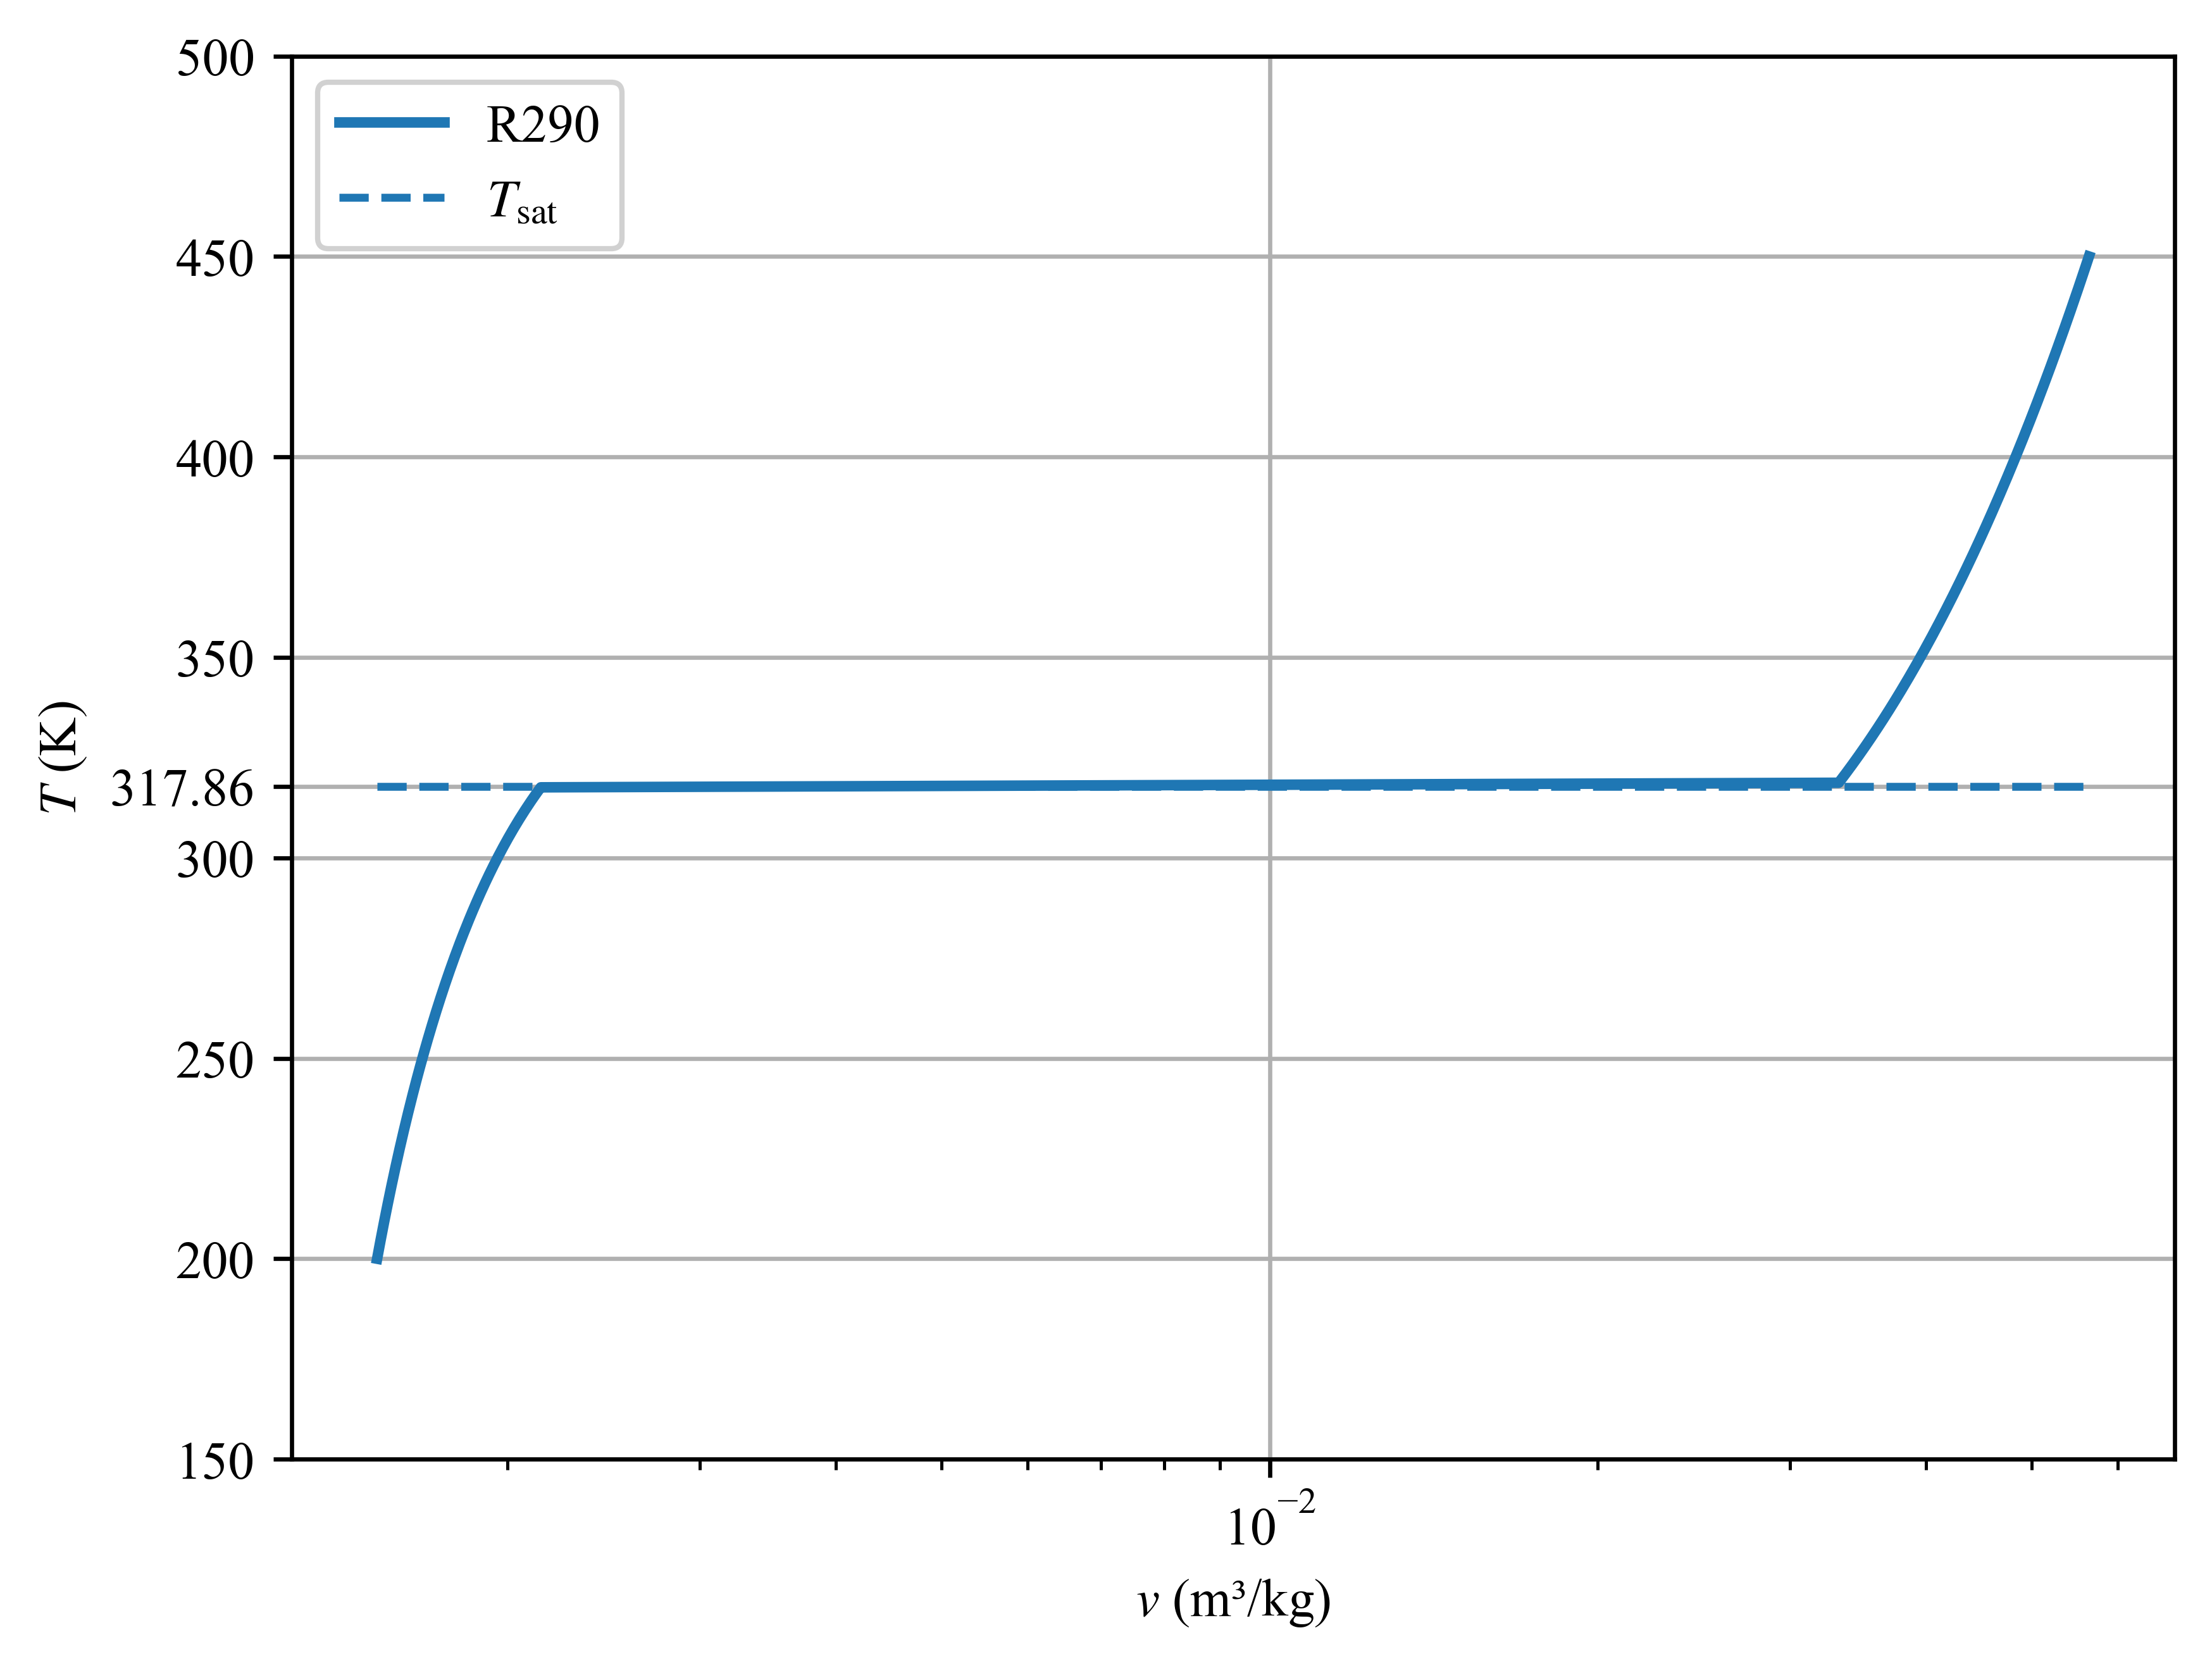
\includegraphics[width=0.7\textwidth]{../chp3/figs/R290.png}
    \caption{R290在1.4MPa下的$T$-$v$图}
\end{figure}

\begin{figure}[H]
    \centering
    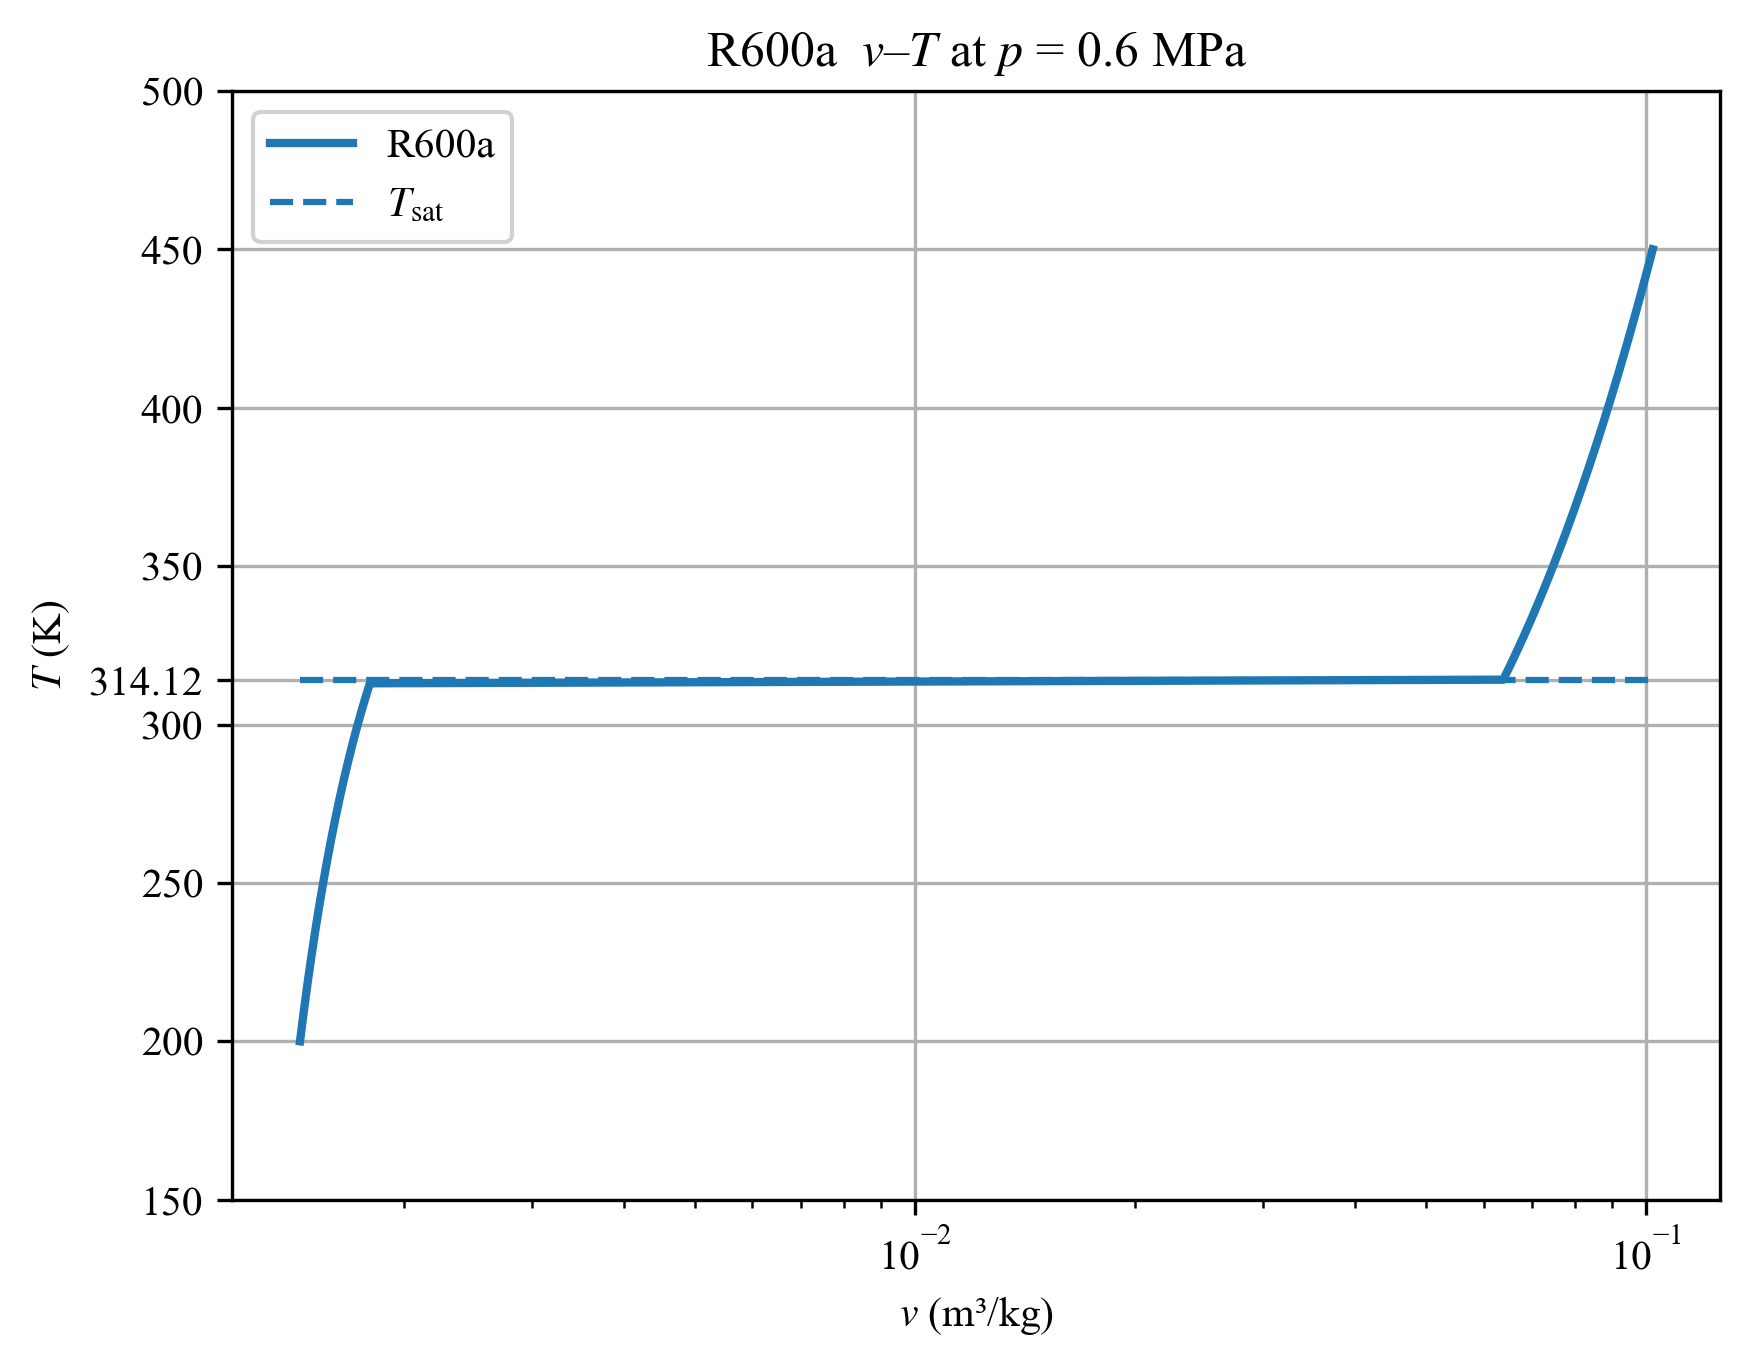
\includegraphics[width=0.7\textwidth]{../chp3/figs/R600a.png}
    \caption{R600a在0.6MPa下的$T$-$v$图}
\end{figure}

程序如下:

\begin{lstlisting}
import numpy as np
import matplotlib.pyplot as plt
import os

# 使用 Times New Roman 作为 matplotlib 全局字体
plt.rcParams["font.family"] = "serif"
plt.rcParams["font.serif"] = ["Times New Roman"]
plt.rcParams["mathtext.fontset"] = "stix"

class PR310:
    def __init__(self, Tc, Pc, omega, M):
        self.Tc = Tc  # 输入K
        self.Pc = Pc * 1e6  # 输入MPa
        self.omega = omega  # 无量纲
        self.M = M / 1000  # 输入g/mol

    R = 8.314462618  # J/(mol*K)

    # 计算a和b
    def params(self, T):
        kappa = 0.37464 + 1.54226 * self.omega - 0.26992 * self.omega**2
        Tr = T / self.Tc
        alpha = (1 + kappa * (1 - Tr**0.5)) ** 2
        a = 0.45724 * self.R**2 * self.Tc**2 / self.Pc * alpha
        b = 0.07780 * self.R * self.Tc / self.Pc
        return a, b

    # 计算A和B
    def AB(self, T, p):
        a, b = self.params(T)
        A = a * p * 1e6 / (self.R * T) ** 2
        B = b * p * 1e6 / (self.R * T)
        return A, B

    # 计算C2, C1, C0
    def C(self, T, p):
        A, B = self.AB(T, p)
        C2 = -(1 - B)
        C1 = A - 3 * B**2 - 2 * B
        C0 = -(A * B - B**2 - B**3)
        return C2, C1, C0

    # 计算压缩因子Z
    # 液相
    def Zl(self, T, p):
        C2, C1, C0 = self.C(T, p)
        # 牛顿法求解Z
        Zl = 0.001  # 初始猜测值
        for _ in range(100):
            f = Zl**3 + C2 * Zl**2 + C1 * Zl + C0
            df = 3 * Zl**2 + 2 * C2 * Zl + C1
            Zl_new = Zl - f / df
            if abs(Zl_new - Zl) < 1e-6:
                break
            Zl = Zl_new
        return Zl

    # 气相
    def Zg(self, T, p):
        C2, C1, C0 = self.C(T, p)
        # 牛顿法求解Z
        Zg = 1.1  # 初始猜测值
        for _ in range(100):
            f = Zg**3 + C2 * Zg**2 + C1 * Zg + C0
            df = 3 * Zg**2 + 2 * C2 * Zg + C1
            Zg_new = Zg - f / df
            if abs(Zg_new - Zg) < 1e-6:
                break
            Zg = Zg_new
        return Zg

    # 计算比体积v
    # 液相
    def vl(self, T, p):
        Zl = self.Zl(T, p)
        vl = Zl * self.R * T / (p * 1e6 * self.M)
        return vl

    # 气相
    def vg(self, T, p):
        Zg = self.Zg(T, p)
        vg = Zg * self.R * T / (p * 1e6 * self.M)
        return vg

    # 画图
    def plot_Tv(
        self,
        fluid_name,  # 流体名称
        p,  # 压力 Pa
        Tsat,  # 饱和温度 K
        T_min,  # 温度范围最小值 K
        T_max,  # 温度范围最大值 K
        nT=220,  # 温度点数
    ):
        T_grid = np.linspace(T_min, T_max, nT)  # 温度网格
        v_grid = np.empty_like(T_grid)  # 比体积网格
        # 计算比体积
        for i, T in enumerate(T_grid):
            if T < Tsat:
                v_grid[i] = self.vl(T, p)
            elif T > Tsat:
                v_grid[i] = self.vg(T, p)
            else:
                v_grid[i] = 0.5 * (self.vl(T, p) + self.vg(T, p))
        fig, ax = plt.subplots()  # 创建图像和坐标轴
        # 主曲线
        ax.plot(v_grid, T_grid, linewidth=2, label=fluid_name)
        xmin, xmax = np.nanmin(v_grid), np.nanmax(v_grid)
        # Tsat 虚线
        ax.hlines(Tsat, xmin, xmax, linestyles="--", label=r"$T_{\mathrm{sat}}$")
        # 标注 Tsat
        yt = list(ax.get_yticks())
        # 加入Tsat并排序
        if not any(abs(t - Tsat) < 1e-8 for t in yt):
            yt.append(Tsat)
        yt = np.array(sorted(yt))
        # 生成刻度标签:对 Tsat 使用仅数值标签(两位小数),其它刻度保留数字格式(根据范围选择小数位)
        deltaT = T_grid.max() - T_grid.min()
        labels = []
        for t in yt:
            if abs(t - Tsat) < 1e-8 or abs(t - Tsat) < 1e-6 * max(1.0, deltaT):
                labels.append(f"{Tsat:.2f}")
            else:
                # 根据温度范围决定格式,避免过多小数
                if deltaT > 50:
                    labels.append(f"{t:.0f}")
                else:
                    labels.append(f"{t:.2f}")
        ax.set_yticks(yt)
        ax.set_yticklabels(labels)
        # 轴标签
        ax.set_xlabel(r"$v$ (m³/kg)")
        ax.set_ylabel(r"$T$ (K)")
        ax.grid(True)
        ax.set_xscale("log")  # 使用对数刻度
        ax.legend(loc="upper left", frameon=True, fancybox=True, framealpha=0.9)

        # 固定保存路径为脚本同目录下的 figs 文件夹
        base_dir = os.path.dirname(os.path.abspath(__file__))
        fig_dir = os.path.join(base_dir, "figs")
        os.makedirs(fig_dir, exist_ok=True)

        # 文件名固定为"流体名称.png"
        filename = f"{fluid_name}.png"
        savepath = os.path.join(fig_dir, filename)

        # 保存图像,固定参数
        fig.savefig(savepath, dpi=600, bbox_inches="tight", transparent=False)
        plt.close(fig)

R290 = PR310(369.89, 4.2512, 0.1521, 44.096)
R290.plot_Tv("R290", 1.4, 317.86, 200, 450)

R600a = PR310(407.81, 3.629, 0.184, 58.122)
R600a.plot_Tv("R600a", 0.6, 314.12, 200, 450)
\end{lstlisting}

\subsection*{3-13}
查物性库得,对于R134a,各参数为:$T_\mathrm{c}=374.21\mathrm{K}$,$p_\mathrm{c}=4.0593\mathrm{MPa}$,$\omega=0.326$,$M=102.03\mathrm{g/mol}$。

对于R1234yf,各参数为:$T_\mathrm{c}=367.85\mathrm{K}$,$p_\mathrm{c}=3.3822\mathrm{MPa}$,$\omega=0.276$,$M=114.04\mathrm{g/mol}$;

对于R1234ze(E),各参数为:$T_\mathrm{c}=382.75\mathrm{K}$,$p_\mathrm{c}=3.6349\mathrm{MPa}$,$\omega=0.313$,$M=114.04\mathrm{g/mol}$;

压力为0.1MPa,温度为35℃=308.15K时,以上三种制冷剂均为气相,调用题3-10中程序计算三种制冷剂的$v_g$。
计算结果为:
$v_\mathrm{R134a}=0.24679\mathrm{m^3/kg}$,$v_\mathrm{R1234yf}=0.22031\mathrm{m^3/kg}$,$v_\mathrm{R1234ze(E)}=0.22007\mathrm{m^3/kg}$

可以看出,三种制冷剂的比体积相差不大,R134a的比体积略大于另外两种,故采用R1234yf和R1234ze(E)作为R134a的替代品是合理的。

程序如下:
\begin{lstlisting}
import PR310 # 导入PR310模块

R134a = PR310.PR310(374.21, 4.0593, 0.326, 102.03)
R1234yf = PR310.PR310(367.85, 3.382, 0.276, 114.04)
R1234zeE = PR310.PR310(382.51, 3.635, 0.313, 114.04)

print(R134a.vg(308.15, 0.1))
print(R1234yf.vg(308.15, 0.1))
print(R1234zeE.vg(308.15, 0.1))
\end{lstlisting}

\subsection*{3-15}

在压力$p=0.1\mathrm{MPa}$、$0.2\mathrm{MPa}$、$0.3\mathrm{MPa}$,温度$T=300\mathrm{K}$时,不同的$k_{ij}$条件下,混合制冷剂R290/R600a的比体积计算结果与计算偏差如表1所示,表中计算偏差是相对于$k_{ij}=0.064$时的比体积计算结果而言的。可以看出,$k_{ij}$取0.1、0和-0.1时,计算结果与$k_{ij}=0.064$时的比体积计算结果偏差逐渐增大,且偏差均小于1\%。
\begin{table}[h]
\centering
\caption{不同$k_{ij}$条件下混合制冷剂R290/R600a的比体积计算结果与计算偏差}
\begin{tabular}{c c c c}
\hline
$p$ (MPa) & $k_{ij}$ &  $v$ (m³/mol) &误差 (\%) \\
\hline
\multirow{4}{*}{0.1} & 0.064 & 0.47838 &   \\
 & 0.1 & 0.47859 & 0.04390\\
 & 0 & 0.47802 & 0.07525  \\
 & -0.1 & 0.47744 & 0.19650  \\
\hline
\multirow{4}{*}{0.2} & 0.064 & 0.23422 &   \\
 & 0.1 & 0.23443 & 0.08966  \\
 & 0 & 0.23384 & 0.16224  \\
 & -0.1 & 0.23324 & 0.41841  \\
\hline
\multirow{4}{*}{0.3} & 0.064 & 0.15273 &   \\
 & 0.1 & 0.15295 & 0.14405  \\
 & 0 & 0.15233 & 0.26190  \\
 & -0.1 & 0.15171 & 0.66785  \\
\hline
\end{tabular}
\end{table}

计算程序如下:

\begin{lstlisting}
class PR315:
    def __init__(self, Tc1, Tc2, pc1, pc2, omega1, omega2, M1, M2, x1, kij):
        self.Tc1 = Tc1  # K
        self.Tc2 = Tc2  # K
        self.pc1 = pc1 * 1e6
        self.pc2 = pc2 * 1e6
        self.omega1 = omega1
        self.omega2 = omega2
        self.M1 = M1 / 1e3
        self.M2 = M2 / 1e3
        self.x1 = x1
        self.x2 = 1 - x1
        self.kij = kij

    R = 8.314462618  # J/(mol*K)

    # 计算a和b
    def params(self, T):
        kappa1 = 0.37464 + 1.54226 * self.omega1 - 0.26992 * self.omega1**2
        kappa2 = 0.37464 + 1.54226 * self.omega2 - 0.26992 * self.omega2**2
        Tr1 = T / self.Tc1
        Tr2 = T / self.Tc2
        alpha1 = (1 + kappa1 * (1 - Tr1**0.5)) ** 2
        alpha2 = (1 + kappa2 * (1 - Tr2**0.5)) ** 2
        a1 = 0.45724 * self.R**2 * self.Tc1**2 / self.pc1 * alpha1
        a2 = 0.45724 * self.R**2 * self.Tc2**2 / self.pc2 * alpha2
        b1 = 0.07780 * self.R * self.Tc1 / self.pc1
        b2 = 0.07780 * self.R * self.Tc2 / self.pc2
        a = (
            self.x1**2 * a1
            + self.x2**2 * a2
            + 2 * self.x1 * self.x2 * (a1 * a2) ** 0.5 * (1 - self.kij)
        )
        b = self.x1 * b1 + self.x2 * b2
        return a, b

    # 计算A和B
    def AB(self, T, p):
        a, b = self.params(T)
        A = a * p * 1e6 / (self.R * T) ** 2
        B = b * p * 1e6 / (self.R * T)
        return A, B

    # 计算C2, C1, C0
    def C(self, T, p):
        A, B = self.AB(T, p)
        C2 = -(1 - B)
        C1 = A - 3 * B**2 - 2 * B
        C0 = -(A * B - B**2 - B**3)
        return C2, C1, C0

    # 计算压缩因子Z
    # 液相
    def Zl(self, T, p):
        C2, C1, C0 = self.C(T, p)
        # 牛顿法求解Z
        Zl = 0.001  # 初始猜测值
        for _ in range(100):
            f = Zl**3 + C2 * Zl**2 + C1 * Zl + C0
            df = 3 * Zl**2 + 2 * C2 * Zl + C1
            Zl_new = Zl - f / df
            if abs(Zl_new - Zl) < 1e-6:
                break
            Zl = Zl_new
        return Zl

    # 气相
    def Zg(self, T, p):
        C2, C1, C0 = self.C(T, p)
        # 牛顿法求解Z
        Zg = 1.1  # 初始猜测值
        for _ in range(100):
            f = Zg**3 + C2 * Zg**2 + C1 * Zg + C0
            df = 3 * Zg**2 + 2 * C2 * Zg + C1
            Zg_new = Zg - f / df
            if abs(Zg_new - Zg) < 1e-6:
                break
            Zg = Zg_new
        return Zg

    # 计算比体积v
    # 液相
    def vl(self, T, p):
        Zl = self.Zl(T, p)
        vl = (
            Zl * self.R * T / (p * 1e6 * (self.x1 * self.M1 + self.x2 * self.M2))
        )  # p从MPa转换为Pa
        return vl

    # 气相
    def vg(self, T, p):
        Zg = self.Zg(T, p)
        vg = (
            Zg * self.R * T / (p * 1e6 * (self.x1 * self.M1 + self.x2 * self.M2))
        )  # p从MPa转换为Pa
        return vg


R290_R600a_1 = PR315(
    369.89, 407.81, 4.2512, 3.629, 0.1521, 0.184, 44.096, 58.122, 0.5, 0.064
)
R290_R600a_2 = PR315(
    369.89, 407.81, 4.2512, 3.629, 0.1521, 0.184, 44.096, 58.122, 0.5, 0.1
)
R290_R600a_3 = PR315(
    369.89, 407.81, 4.2512, 3.629, 0.1521, 0.184, 44.096, 58.122, 0.5, 0
)
R290_R600a_4 = PR315(
    369.89, 407.81, 4.2512, 3.629, 0.1521, 0.184, 44.096, 58.122, 0.5, -0.1
)
print(R290_R600a_1.vg(300, 0.1))
print(R290_R600a_2.vg(300, 0.1))
print(R290_R600a_3.vg(300, 0.1))
print(R290_R600a_4.vg(300, 0.1))
print(R290_R600a_1.vg(300, 0.2))
print(R290_R600a_2.vg(300, 0.2))
print(R290_R600a_3.vg(300, 0.2))
print(R290_R600a_4.vg(300, 0.2))
print(R290_R600a_1.vg(300, 0.3))
print(R290_R600a_2.vg(300, 0.3))
print(R290_R600a_3.vg(300, 0.3))
print(R290_R600a_4.vg(300, 0.3))
\end{lstlisting}

\newpage

\section*{第四章}

\subsection*{4-13}

利用主程序分别计算在1.4MPa下不同温度$T$下R290的液相焓和熵,以及在0.6MPa下不同温度$T$下R600a的液相焓和熵,计算结果与标准值对比如表2和表3所示,可以看出,计算结果与标准值误差均小于1\%。

\begin{table}[h]
\centering
\caption{1.4MPa下不同温度$T$下R290的液相焓和熵计算结果与标准值对比}
\begin{tabular}{c c c c c c c}
\hline
$T$ (K) & $h$ (kJ/kg) &$h_\text{标准}$(kJ/kg) & $s$ (kJ/(kg·K)) &$s_\text{标准}$(kJ/(kg·K))& $h$误差\%&$s$误差\%\\
\hline
260 & 168.686& 170.083& 0.876& 0.881& 0.821& 0.567\\
270 & 192.542& 194.346& 0.966& 0.973& 0.928& 0.719\\
280 & 217.443& 219.262& 1.057& 1.063& 0.830& 0.723\\
290 & 243.544& 244.914& 1.149& 1.153& 0.559& 0.347\\
300 & 271.043& 271.376& 1.242& 1.243& 0.123& 0.080\\
\hline
\end{tabular}
\end{table}

\begin{table}[h]
\centering
\caption{0.6MPa下不同温度$T$下R600a的液相焓和熵计算结果与标准值对比}
\begin{tabular}{c c c c c c c}
\hline
$T$ (K) & $h$ (kJ/kg) &$h_\text{标准}$(kJ/kg) & $s$ (kJ/(kg·K)) &$s_\text{标准}$(kJ/(kg·K))& $h$误差\%&$s$误差\%\\
\hline
260 & 171.745& 171.556& 0.891& 0.891& 0.110& 0\\
270 & 193.349& 193.946& 0.973& 0.975& 0.308& 0.205\\
280 & 215.677& 216.839& 1.054& 1.058& 0.536& 0.378\\
290 & 238.773& 240.279& 1.135& 1.140& 0.627& 0.438\\
300 & 262.694& 264.277& 1.216& 1.222& 0.158& 0.491\\
\hline
\end{tabular}
\end{table}

程序如下:
\begin{lstlisting}
import numpy as np

class PR413:
    def __init__(self, Tc, pc, omega, M, ps0):
        self.Tc = Tc  # K
        self.pc = pc * 1e6
        self.omega = omega
        self.M = M / 1e3
        self.ps0 = ps0

    R = 8.314462618  # J/(mol*K)

    # 计算a和b
    def params(self, T):
        kappa = 0.37464 + 1.54226 * self.omega - 0.26992 * self.omega**2
        Tr = T / self.Tc
        alpha = (1 + kappa * (1 - Tr**0.5)) ** 2
        a = 0.45724 * self.R**2 * self.Tc**2 / self.pc * alpha
        da = (
            -0.45724
            * self.R**2
            * self.Tc**2
            / self.pc
            * kappa
            * (1 + kappa * (1 - Tr**0.5))
            * (Tr**-0.5)
            / self.Tc
        )
        b = 0.07780 * self.R * self.Tc / self.pc
        return a, b, da

    # 计算A和B
    def AB(self, T, p):
        a, b, da = self.params(T)
        A = a * p * 1e6 / (self.R * T) ** 2
        B = b * p * 1e6 / (self.R * T)
        return A, B

    # 计算C2, C1, C0
    def C(self, T, p):
        A, B = self.AB(T, p)
        C2 = -(1 - B)
        C1 = A - 3 * B**2 - 2 * B
        C0 = -(A * B - B**2 - B**3)
        return C2, C1, C0

    # 计算压缩因子Z
    # 液相
    def Zl(self, T, p):
        C2, C1, C0 = self.C(T, p)
        # 牛顿法求解Z
        Zl = 0.001  # 初始猜测值
        for _ in range(100):
            f = Zl**3 + C2 * Zl**2 + C1 * Zl + C0
            df = 3 * Zl**2 + 2 * C2 * Zl + C1
            Zl_new = Zl - f / df
            if abs(Zl_new - Zl) < 1e-6:
                break
            Zl = Zl_new
        return Zl

    # 气相
    def Zg(self, T, p):
        C2, C1, C0 = self.C(T, p)
        # 牛顿法求解Z
        Zg = 1.1  # 初始猜测值
        for _ in range(100):
            f = Zg**3 + C2 * Zg**2 + C1 * Zg + C0
            df = 3 * Zg**2 + 2 * C2 * Zg + C1
            Zg_new = Zg - f / df
            if abs(Zg_new - Zg) < 1e-6:
                break
            Zg = Zg_new
        return Zg

    # 计算比体积v
    # 液相
    def vl(self, T, p):
        Zl = self.Zl(T, p)
        vl = Zl * self.R * T / (p * 1e6)
        return vl

    # 气相
    def vg(self, T, p):
        Zg = self.Zg(T, p)
        vg = Zg * self.R * T / (p * 1e6)
        return vg

    # 计算焓的余函数
    # 液相
    def h_res_l(self, T, p):
        a, b, da = self.params(T)
        Zl = self.Zl(T, p)
        vl = self.vl(T, p)
        hr_l = (T * da - a) / (b * np.sqrt(8)) * np.log(
            (vl - 0.414 * b) / (vl + 2.414 * b)
        ) + self.R * T * (1 - Zl)
        return hr_l

    # 气相
    def h_res_g(self, T, p):
        a, b, da = self.params(T)
        Zg = self.Zg(T, p)
        vg = self.vg(T, p)
        hr_g = (T * da - a) / (b * np.sqrt(8)) * np.log(
            (vg - 0.414 * b) / (vg + 2.414 * b)
        ) + self.R * T * (1 - Zg)
        return hr_g

    # 计算熵的余函数
    # 液相
    def s_res_l(self, T, p):
        a, b, da = self.params(T)
        vl = self.vl(T, p)
        sr_l = (
            -self.R * np.log((vl - b) / vl)
            - self.R * np.log(vl / (self.R * T / (p * 1e6)))
            + da / (b * np.sqrt(8)) * np.log((vl - 0.414 * b) / (vl + 2.414 * b))
        )
        return sr_l

    # 气相
    def s_res_g(self, T, p):
        a, b, da = self.params(T)
        vg = self.vg(T, p)
        sr_g = (
            -self.R * np.log((vg - b) / vg)
            - self.R * np.log(vg / (self.R * T / (p * 1e6)))
            + da / (b * np.sqrt(8)) * np.log((vg - 0.414 * b) / (vg + 2.414 * b))
        )
        return sr_g

    # 计算c_p积分
    def cp(self, T, A, B, C, D):
        cp = (
            A * (T - 273.15)
            + B / 2 * (T**2 - 273.15**2)
            + C / 3 * (T**3 - 273.15**3)
            + D / 4 * (T**4 - 273.15**4)
        )
        return cp

    # 计算c_p/T积分
    def cpT(self, T, A, B, C, D):
        cp = (
            A * np.log(T / 273.15)
            + B * (T - 273.15)
            + C / 2 * (T**2 - 273.15**2)
            + D / 3 * (T**3 - 273.15**3)
        )
        return cp

    # 计算焓和熵
    # 液相
    def h_l(self, T, A, B, C, D, p):
        h_r_ps_0 = self.h_res_l(273.15, self.ps0)
        cp0 = self.cp(T, A, B, C, D)
        h_res_l = self.h_res_l(T, p)
        hl = 200 * 1e3 + cp0 + (h_r_ps_0 - h_res_l) / self.M  # J/kg
        return hl

    def s_l(self, T, A, B, C, D, p):
        s_r_ps_0 = self.s_res_l(273.15, self.ps0)
        cpT = self.cpT(T, A, B, C, D)
        sr_l = self.s_res_l(T, p)
        sl = (
            1e3 + cpT + (s_r_ps_0 - self.R * np.log(p / self.ps0) - sr_l) / self.M
        )  # J/(kg*K)
        return sl

    # 气相
    def h_g(self, T, A, B, C, D, p):
        h_r_ps_0 = self.h_res_l(273.15, self.ps0)  # 使用液相作为基准
        cp0 = self.cp(T, A, B, C, D)
        h_res_g = self.h_res_g(T, p)
        hg = 200 * 1e3 + cp0 + (h_r_ps_0 - h_res_g) / self.M  # J/kg
        return hg

    def s_g(self, T, A, B, C, D, p):
        s_r_ps_0 = self.s_res_l(273.15, self.ps0)  # 使用液相作为基准
        cpT = self.cpT(T, A, B, C, D)
        sr_g = self.s_res_g(T, p)
        sg = (
            1e3 + cpT + (s_r_ps_0 - self.R * np.log(p / self.ps0) - sr_g) / self.M
        )  # J/(kg*K)
        return sg


R290 = PR413(369.89, 4.2512, 0.1521, 44.096, 0.47446)
R600a = PR413(407.81, 3.629, 0.184, 58.122, 0.15696)

print(R290.h_l(300, -95.80, 6.945, -3.597 * 1e-3, 7.290 * 1e-7, 1.4))
print(R290.s_l(300, -95.80, 6.945, -3.597 * 1e-3, 7.290 * 1e-7, 1.4))
print(R600a.h_l(300, -23.91, 6.605, -3.176 * 1e-3, 4.981 * 1e-7, 0.6))
print(R600a.s_l(300, -23.91, 6.605, -3.176 * 1e-3, 4.981 * 1e-7, 0.6))
\end{lstlisting}

\subsection*{4-15}
取二元作用系数$k_{ij}=0.064$,在$p$=1.0MPa下不同温度下计算R290/R600a(50\%/50\%)混合制冷剂的焓和熵,计算结果如表4所示,结果表明,计算结果与标准值误差很小。

\begin{table}[h]
\centering
\caption{1.0MPa下不同温度$T$下R290/R600a(50\%/50\%)混合制冷剂的液相焓和熵计算结果与标准值对比}
\begin{tabular}{c c c c c c c}
\hline
$T$ (K) & $h$ (kJ/kg) &$h_\text{标准}$(kJ/kg) & $s$ (kJ/(kg·K)) &$s_\text{标准}$(kJ/(kg·K))& $h$误差\%&$s$误差\%\\
\hline
260 & 170.450& 170.056& 0.885& 0.889& 0.232& 0.450\\
270 & 193.011& 193.144& 0.970& 0.979& 0.069& 0.919\\
280 & 216.459& 216.813& 1.055& 1.066& 0.163& 1.032\\
290 & 240.885& 241.124& 1.141& 1.150& 0.099& 0.783\\
300 & 266.428& 266.154& 1.228& 1.231& 0.103& 0.244\\
\hline
\end{tabular}
\end{table}

程序如下:
\begin{lstlisting}
import numpy as np

class PR415:
    def __init__(self, Tc1, pc1, omega1, M1, x1, Tc2, pc2, omega2, M2, kij, ps0):
        self.Tc1 = Tc1  # K
        self.pc1 = pc1 * 1e6
        self.omega1 = omega1
        self.M1 = M1 / 1e3
        self.x1 = x1

        self.Tc2 = Tc2  # K
        self.pc2 = pc2 * 1e6
        self.omega2 = omega2
        self.M2 = M2 / 1e3
        self.x2 = 1 - x1

        self.ps0 = ps0

        self.kij = kij

    R = 8.314462618  # J/(mol*K)

    # 计算a和b
    def params(self, T):
        kappa1 = 0.37464 + 1.54226 * self.omega1 - 0.26992 * self.omega1**2
        kappa2 = 0.37464 + 1.54226 * self.omega2 - 0.26992 * self.omega2**2
        Tr1 = T / self.Tc1
        Tr2 = T / self.Tc2
        alpha1 = (1 + kappa1 * (1 - Tr1**0.5)) ** 2
        alpha2 = (1 + kappa2 * (1 - Tr2**0.5)) ** 2
        a1 = 0.45724 * self.R**2 * self.Tc1**2 / self.pc1 * alpha1
        a2 = 0.45724 * self.R**2 * self.Tc2**2 / self.pc2 * alpha2
        da1 = (
            -0.45724
            * self.R**2
            * self.Tc1**2
            / self.pc1
            * kappa1
            * (1 + kappa1 * (1 - Tr1**0.5))
            * (Tr1**-0.5)
            / self.Tc1
        )
        da2 = (
            -0.45724
            * self.R**2
            * self.Tc2**2
            / self.pc2
            * kappa2
            * (1 + kappa2 * (1 - Tr2**0.5))
            * (Tr2**-0.5)
            / self.Tc2
        )
        b1 = 0.07780 * self.R * self.Tc1 / self.pc1
        b2 = 0.07780 * self.R * self.Tc2 / self.pc2

        a = (
            self.x1**2 * a1
            + self.x2**2 * a2
            + 2 * self.x1 * self.x2 * (a1 * a2) ** 0.5 * (1 - self.kij)
        )
        b = self.x1 * b1 + self.x2 * b2
        da = (
            self.x1**2 * da1
            + self.x2**2 * da2
            + self.x1
            * self.x2
            * (1 - self.kij)
            * ((a2 / a1) ** 0.5 * da1 + (a1 / a2) ** 0.5 * da2)
        )
        return a, b, da

    # 计算A和B
    def AB(self, T, p):
        a, b, da = self.params(T)
        A = a * p * 1e6 / (self.R * T) ** 2
        B = b * p * 1e6 / (self.R * T)
        return A, B

    # 计算C2, C1, C0
    def C(self, T, p):
        A, B = self.AB(T, p)
        C2 = -(1 - B)
        C1 = A - 3 * B**2 - 2 * B
        C0 = -(A * B - B**2 - B**3)
        return C2, C1, C0

    # 计算压缩因子Z
    # 液相
    def Zl(self, T, p):
        C2, C1, C0 = self.C(T, p)
        # 牛顿法求解Z
        Zl = 0.001  # 初始猜测值
        for _ in range(100):
            f = Zl**3 + C2 * Zl**2 + C1 * Zl + C0
            df = 3 * Zl**2 + 2 * C2 * Zl + C1
            Zl_new = Zl - f / df
            if abs(Zl_new - Zl) < 1e-6:
                break
            Zl = Zl_new
        return Zl

    # 气相
    def Zg(self, T, p):
        C2, C1, C0 = self.C(T, p)
        # 牛顿法求解Z
        Zg = 1.1  # 初始猜测值
        for _ in range(100):
            f = Zg**3 + C2 * Zg**2 + C1 * Zg + C0
            df = 3 * Zg**2 + 2 * C2 * Zg + C1
            Zg_new = Zg - f / df
            if abs(Zg_new - Zg) < 1e-6:
                break
            Zg = Zg_new
        return Zg

    # 计算比体积v
    # 液相
    def vl(self, T, p):
        Zl = self.Zl(T, p)
        vl = Zl * self.R * T / (p * 1e6)
        return vl

    # 气相
    def vg(self, T, p):
        Zg = self.Zg(T, p)
        vg = Zg * self.R * T / (p * 1e6)
        return vg

    # 计算焓的余函数
    # 液相
    def h_res_l(self, T, p):
        a, b, da = self.params(T)
        Zl = self.Zl(T, p)
        vl = self.vl(T, p)
        hr_l = (T * da - a) / (b * np.sqrt(8)) * np.log(
            (vl - 0.414 * b) / (vl + 2.414 * b)
        ) + self.R * T * (1 - Zl)
        return hr_l

    # 气相
    def h_res_g(self, T, p):
        a, b, da = self.params(T)
        Zg = self.Zg(T, p)
        vg = self.vg(T, p)
        hr_g = (T * da - a) / (b * np.sqrt(8)) * np.log(
            (vg - 0.414 * b) / (vg + 2.414 * b)
        ) + self.R * T * (1 - Zg)
        return hr_g

    # 计算熵的余函数
    # 液相
    def s_res_l(self, T, p):
        a, b, da = self.params(T)
        vl = self.vl(T, p)
        sr_l = (
            -self.R * np.log((vl - b) / vl)
            - self.R * np.log(vl / (self.R * T / (p * 1e6)))
            + da / (b * np.sqrt(8)) * np.log((vl - 0.414 * b) / (vl + 2.414 * b))
        )
        return sr_l

    # 气相
    def s_res_g(self, T, p):
        a, b, da = self.params(T)
        vg = self.vg(T, p)
        sr_g = (
            -self.R * np.log((vg - b) / vg)
            - self.R * np.log(vg / (self.R * T / (p * 1e6)))
            + da / (b * np.sqrt(8)) * np.log((vg - 0.414 * b) / (vg + 2.414 * b))
        )
        return sr_g

    # 计算c_p积分
    def cp(self, T, A1, A2, B1, B2, C1, C2, D1, D2):
        cp = (
            (A1 + A2) * 0.5 * (T - 273.15)
            + (B1 + B2) * 0.5 / 2 * (T**2 - 273.15**2)
            + (C1 + C2) * 0.5 / 3 * (T**3 - 273.15**3)
            + (D1 + D2) * 0.5 / 4 * (T**4 - 273.15**4)
        )
        return cp

    # 计算c_p/T积分
    def cpT(self, T, A1, A2, B1, B2, C1, C2, D1, D2):
        cp = (
            (A1 + A2) * 0.5 * np.log(T / 273.15)
            + (B1 + B2) * 0.5 * (T - 273.15)
            + (C1 + C2) * 0.5 / 2 * (T**2 - 273.15**2)
            + (D1 + D2) * 0.5 / 3 * (T**3 - 273.15**3)
        )
        return cp

    # 计算焓和熵
    # 液相
    def h_l(self, T, A1, A2, B1, B2, C1, C2, D1, D2, p):
        h_r_ps_0 = self.h_res_l(273.15, self.ps0)
        cp0 = self.cp(T, A1, A2, B1, B2, C1, C2, D1, D2)
        h_res_l = self.h_res_l(T, p)
        hl = (
            200 * 1e3
            + cp0
            + (h_r_ps_0 - h_res_l) / (self.x1 * self.M1 + self.x2 * self.M2)
        )  # J/kg
        return hl

    def s_l(self, T, A1, A2, B1, B2, C1, C2, D1, D2, p):
        s_r_ps_0 = self.s_res_l(273.15, self.ps0)
        cpT = self.cpT(T, A1, A2, B1, B2, C1, C2, D1, D2)
        sr_l = self.s_res_l(T, p)
        sl = (
            1e3
            + cpT
            + (s_r_ps_0 - self.R * np.log(p / self.ps0) - sr_l)
            / (self.x1 * self.M1 + self.x2 * self.M2)
        )  # J/(kg*K)
        return sl

    # 气相
    def h_g(self, T, A1, A2, B1, B2, C1, C2, D1, D2, p):
        h_r_ps_0 = self.h_res_l(273.15, self.ps0)  # 使用液相作为基准
        cp0 = self.cp(T, A1, A2, B1, B2, C1, C2, D1, D2)
        h_res_g = self.h_res_g(T, p)
        hg = (
            200 * 1e3
            + cp0
            + (h_r_ps_0 - h_res_g) / (self.x1 * self.M1 + self.x2 * self.M2)
        )  # J/kg
        return hg

    def s_g(self, T, A1, A2, B1, B2, C1, C2, D1, D2, p):
        s_r_ps_0 = self.s_res_l(273.15, self.ps0)  # 使用液相作为基准
        cpT = self.cpT(T, A1, A2, B1, B2, C1, C2, D1, D2)
        sr_g = self.s_res_g(T, p)
        sg = (
            1e3
            + cpT
            + (s_r_ps_0 - self.R * np.log(p / self.ps0) - sr_g)
            / (self.x1 * self.M1 + self.x2 * self.M2)
        )  # J/(kg*K)
        return sg


R290R600a = PR415(
    Tc1=369.89,
    pc1=4.2512,
    omega1=0.1521,
    M1=44.096,  # R290
    x1=0.5,
    Tc2=407.81,
    pc2=3.629,
    omega2=0.184,
    M2=58.122,  # R600a
    kij=0.064,
    ps0=0.32979,
)

# 300K下计算比焓和比熵  
print(
    R290R600a.h_l(
        300,
        -95.80,
        -23.91,
        6.945,
        6.605,
        -3.597 * 1e-3,
        -3.176 * 1e-3,
        7.290 * 1e-7,
        4.981 * 1e-7,
        1.0,
    )
)
print(
    R290R600a.s_l(
        300,
        -95.80,
        -23.91,
        6.945,
        6.605,
        -3.597 * 1e-3,
        -3.176 * 1e-3,
        7.290 * 1e-7,
        4.981 * 1e-7,
        1.0,
    )
)
\end{lstlisting}

\subsection*{6-11}

推导过程见作业手写部分,1.4MPa下R290/R600a混合制冷剂的$\hat{\phi}$-$T$图和$\hat{f}$-$T$图如下:
\begin{figure}[H]
    \centering
    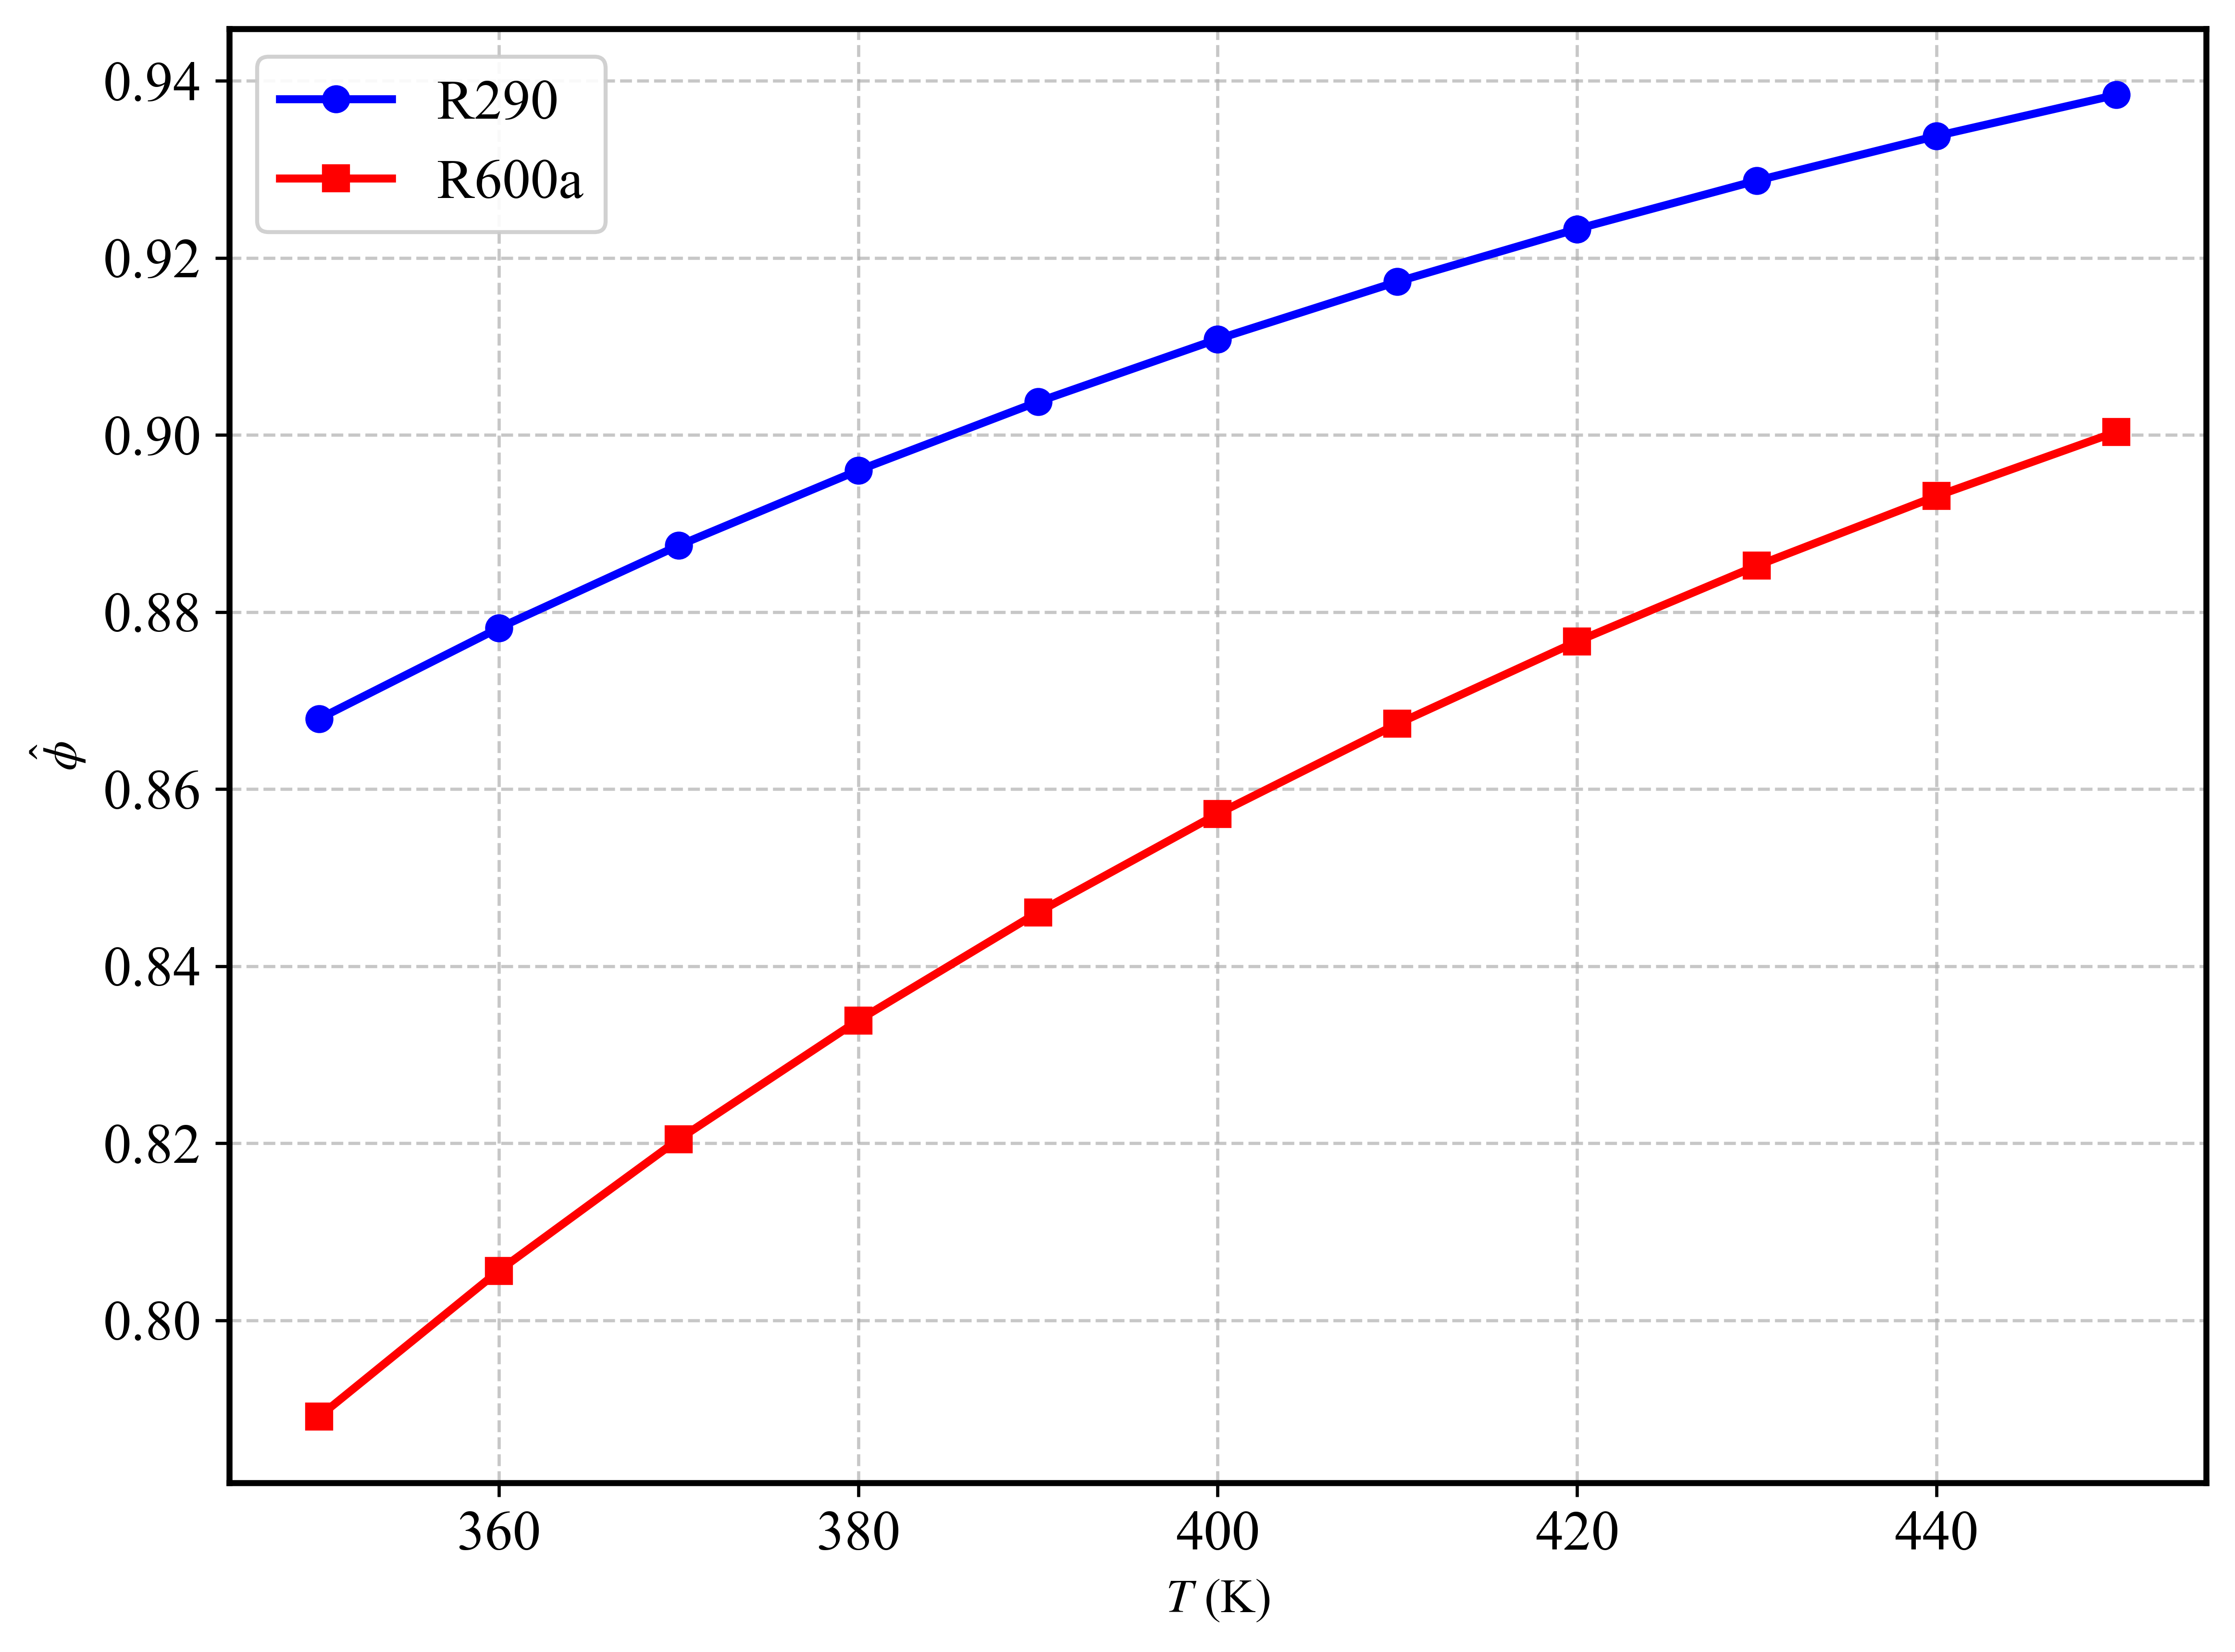
\includegraphics[width=0.7\textwidth]{../chp6/figs/R290R600a_phi.png}
    \caption{1.4MPa下R290/R600a混合制冷剂的$\hat{\phi}$-$T$图}
\end{figure}

\begin{figure}[H]
    \centering
    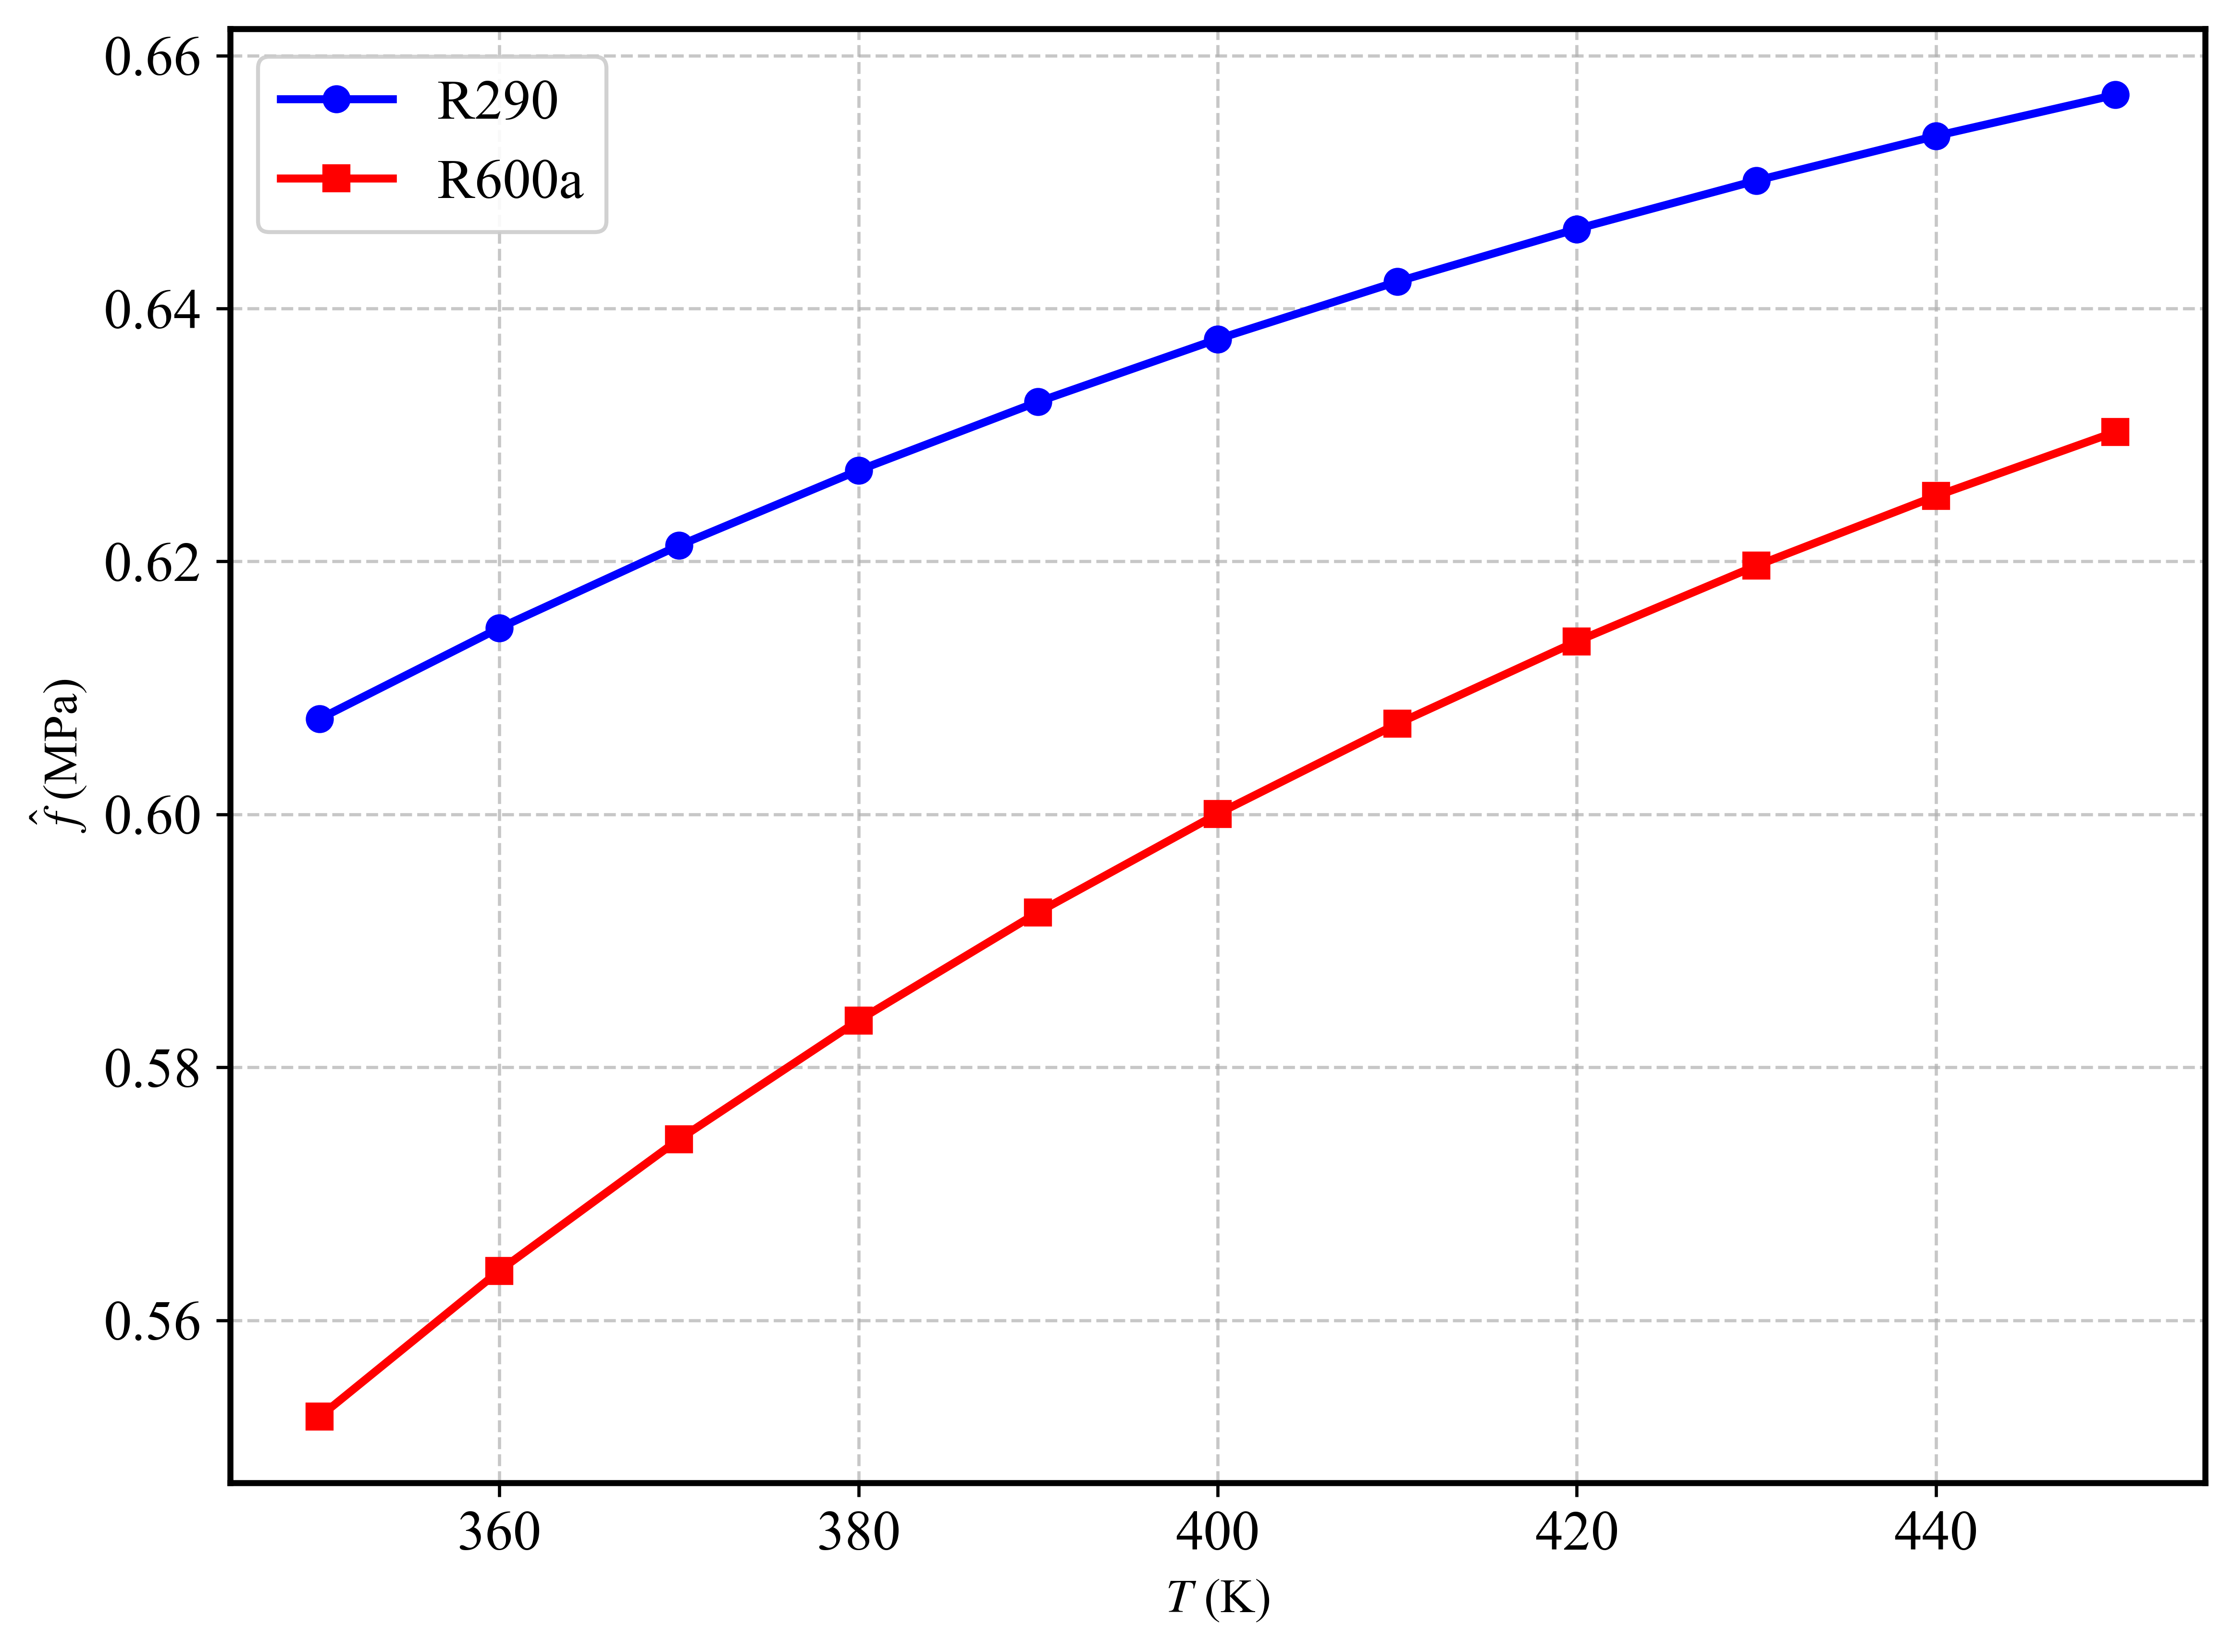
\includegraphics[width=0.7\textwidth]{../chp6/figs/R290R600a_f.png}
    \caption{1.4MPa下R290/R600a混合制冷剂的$\hat{f}$-$T$图}
\end{figure}

程序如下:
\begin{lstlisting}
import numpy as np
import matplotlib.pyplot as plt
import os

# 使用 Times New Roman 作为 matplotlib 全局字体
plt.rcParams["font.family"] = "serif"
plt.rcParams["font.serif"] = ["Times New Roman"]
plt.rcParams["mathtext.fontset"] = "stix"
plt.rcParams["font.size"] = 14  # 增大全局字体
plt.rcParams["axes.linewidth"] = 1.5  # 增粗坐标轴


class PR611:
    def __init__(self, Tc1, pc1, omega1, Tc2, pc2, omega2, x1, kij):
        self.Tc1 = Tc1
        self.pc1 = pc1 * 1e6
        self.omega1 = omega1
        self.Tc2 = Tc2
        self.pc2 = pc2 * 1e6
        self.omega2 = omega2
        self.x1 = x1
        self.x2 = 1 - x1
        self.kij = kij

    R = 8.314462618  # J/(mol·K)

    # 计算a和b
    def params(self, T):
        kappa1 = 0.37464 + 1.54226 * self.omega1 - 0.26992 * self.omega1**2
        kappa2 = 0.37464 + 1.54226 * self.omega2 - 0.26992 * self.omega2**2
        Tr1 = T / self.Tc1
        Tr2 = T / self.Tc2
        alpha1 = (1 + kappa1 * (1 - Tr1**0.5)) ** 2
        alpha2 = (1 + kappa2 * (1 - Tr2**0.5)) ** 2
        a1 = 0.45724 * self.R**2 * self.Tc1**2 / self.pc1 * alpha1
        a2 = 0.45724 * self.R**2 * self.Tc2**2 / self.pc2 * alpha2
        da1 = (
            -0.45724
            * self.R**2
            * self.Tc1**2
            / self.pc1
            * kappa1
            * (1 + kappa1 * (1 - Tr1**0.5))
            * (Tr1**-0.5)
            / self.Tc1
        )
        da2 = (
            -0.45724
            * self.R**2
            * self.Tc2**2
            / self.pc2
            * kappa2
            * (1 + kappa2 * (1 - Tr2**0.5))
            * (Tr2**-0.5)
            / self.Tc2
        )
        b1 = 0.07780 * self.R * self.Tc1 / self.pc1
        b2 = 0.07780 * self.R * self.Tc2 / self.pc2

        a = (
            self.x1**2 * a1
            + self.x2**2 * a2
            + 2 * self.x1 * self.x2 * (a1 * a2) ** 0.5 * (1 - self.kij)
        )
        b = self.x1 * b1 + self.x2 * b2
        da = (
            self.x1**2 * da1
            + self.x2**2 * da2
            + self.x1
            * self.x2
            * (1 - self.kij)
            * ((a2 / a1) ** 0.5 * da1 + (a1 / a2) ** 0.5 * da2)
        )
        return a1, a2, a, b1, b2, b, da

    # 计算A和B
    def AB(self, T, p):
        a1, a2, a, b1, b2, b, da = self.params(T)
        A = a * p * 1e6 / (self.R * T) ** 2
        B = b * p * 1e6 / (self.R * T)
        return A, B

    # 计算C2,C1,C0
    def C(self, T, p):
        A, B = self.AB(T, p)
        C2 = -(1 - B)
        C1 = A - 3 * B**2 - 2 * B
        C0 = -(A * B - B**2 - B**3)
        return C2, C1, C0

    # 计算压缩因子Z
    # 气相
    def Zg(self, T, p):
        C2, C1, C0 = self.C(T, p)
        # 牛顿法求解Z
        Zg = 1.1  # 初始猜测值
        for _ in range(100):
            f = Zg**3 + C2 * Zg**2 + C1 * Zg + C0
            df = 3 * Zg**2 + 2 * C2 * Zg + C1
            Zg_new = Zg - f / df
            if abs(Zg_new - Zg) < 1e-6:
                break
            Zg = Zg_new
        return Zg

    # 计算比体积v
    # 气相
    def vg(self, T, p):
        Zg = self.Zg(T, p)
        vg = Zg * self.R * T / (p * 1e6)
        return vg  # m³/mol

    # 计算逸度系数
    # 气相
    def phi_g(self, T, p):
        Zg = self.Zg(T, p)
        a1, a2, a, b1, b2, b, da = self.params(T)
        A, B = self.AB(T, p)
        phi_g1 = np.exp(
            (b1 / b) * (Zg - 1)
            - np.log(Zg - B)
            - A
            / (B * np.sqrt(8))
            * (
                2 * (self.x2 * (1 - self.kij) * (a1 * a2) ** 0.5 + self.x1 * a1) / a
                - b1 / b
            )
            * np.log((Zg + 2.414 * B) / (Zg - 0.414 * B))
        )
        phi_g2 = np.exp(
            (b2 / b) * (Zg - 1)
            - np.log(Zg - B)
            - A
            / (B * np.sqrt(8))
            * (
                2 * (self.x1 * (1 - self.kij) * (a1 * a2) ** 0.5 + self.x2 * a2) / a
                - b2 / b
            )
            * np.log((Zg + 2.414 * B) / (Zg - 0.414 * B))
        )
        return phi_g1, phi_g2

    # 计算逸度
    # 气相
    def f_g(self, T, p):  # MPa
        phi_g1, phi_g2 = self.phi_g(T, p)
        f_g1 = self.x1 * phi_g1 * p
        f_g2 = self.x2 * phi_g2 * p
        return f_g1, f_g2

    # 绘制溶液气相f-T、phi-T图
    def plot_fT(self, fluid_name, p, T_min, T_max, nT=11):
        T_grid = np.linspace(T_min, T_max, nT)  # 温度网格
        phi_grid1 = np.empty_like(T_grid)  # 组分1逸度系数网格
        phi_grid2 = np.empty_like(T_grid)  # 组分2逸度系数网格
        f_grid1 = np.empty_like(T_grid)  # 组分1逸度网格
        f_grid2 = np.empty_like(T_grid)  # 组分2逸度网格

        base_dir = os.path.dirname(os.path.abspath(__file__))
        fig_dir = os.path.join(base_dir, "figs")
        os.makedirs(fig_dir, exist_ok=True)

        # 计算逸度系数和逸度
        for i, T in enumerate(T_grid):
            phi_g1, phi_g2 = self.phi_g(T, p)
            f_g1, f_g2 = self.f_g(T, p)
            phi_grid1[i] = phi_g1
            phi_grid2[i] = phi_g2
            f_grid1[i] = f_g1
            f_grid2[i] = f_g2

        # T-phi图
        fig_phi = plt.figure(figsize=(8, 6))
        ax_phi = fig_phi.add_subplot(1, 1, 1)
        ax_phi.plot(T_grid, phi_grid1, "b-o", linewidth=2, label="R290", markersize=6)
        ax_phi.plot(T_grid, phi_grid2, "r-s", linewidth=2, label="R600a", markersize=6)
        ax_phi.set_xlabel(r"$T$ (K)", fontsize=12)
        ax_phi.set_ylabel(r"$\hat{\phi}$", fontsize=12)
        ax_phi.grid(True, linestyle="--", alpha=0.7)
        ax_phi.legend(loc="best", frameon=True, fancybox=True, framealpha=0.9)
        fig_phi.tight_layout()
        savepath_phi = os.path.join(fig_dir, f"{fluid_name}_phi.png")
        fig_phi.savefig(savepath_phi, dpi=600, bbox_inches="tight", transparent=False)
        plt.close(fig_phi)

        # T-f图
        fig_f = plt.figure(figsize=(8, 6))
        ax_f = fig_f.add_subplot(111)
        ax_f.plot(T_grid, f_grid1, "b-o", linewidth=2, label="R290", markersize=6)
        ax_f.plot(T_grid, f_grid2, "r-s", linewidth=2, label="R600a", markersize=6)
        ax_f.set_xlabel(r"$T$ (K)", fontsize=12)
        ax_f.set_ylabel(r"$\hat{f}$ (MPa)", fontsize=12)
        ax_f.grid(True, linestyle="--", alpha=0.7)
        ax_f.legend(loc="best", frameon=True, fancybox=True, framealpha=0.9)
        fig_f.tight_layout()
        savepath_f = os.path.join(fig_dir, f"{fluid_name}_f.png")
        fig_f.savefig(savepath_f, dpi=600, bbox_inches="tight", transparent=False)
        plt.close(fig_f)


R290R600a = PR611(
    Tc1=369.89,
    pc1=4.2512,
    omega1=0.1521,
    Tc2=407.81,
    pc2=3.629,
    omega2=0.184,
    x1=0.5,
    kij=0.064,
)

R290R600a.plot_fT("R290R600a", 1.4, 350, 450, 11)
\end{lstlisting}

\subsection*{7-3}
式(7.13)为:
\begin{equation*}
    \ln p_\mathrm{r} = \ln T_\mathrm{r}[A_1+A_2 \tau^{1.89}+A_3 \tau^{5.67}]
\end{equation*}
其中$p_\mathrm{r}=p/p_\mathrm{c}$,$T_\mathrm{r}=T/T_\mathrm{c}$,$\tau=1-T_\mathrm{r}$。整理得:
\begin{equation*}
    p = p_\mathrm{c} (\frac{T}{T_\mathrm{c}})^{A_1+A_2 (1-\frac{T}{T_\mathrm{c}})^{1.89}+A_3 (1-\frac{T}{T_\mathrm{c}})^{5.67}}
\end{equation*}
由书中表7.1可知甲烷、乙烷、丙烷和丁烷项-谭方程的相关常数,带入求解。绘制的蒸汽压曲线如下图所示:
\begin{figure}[H]
    \centering
    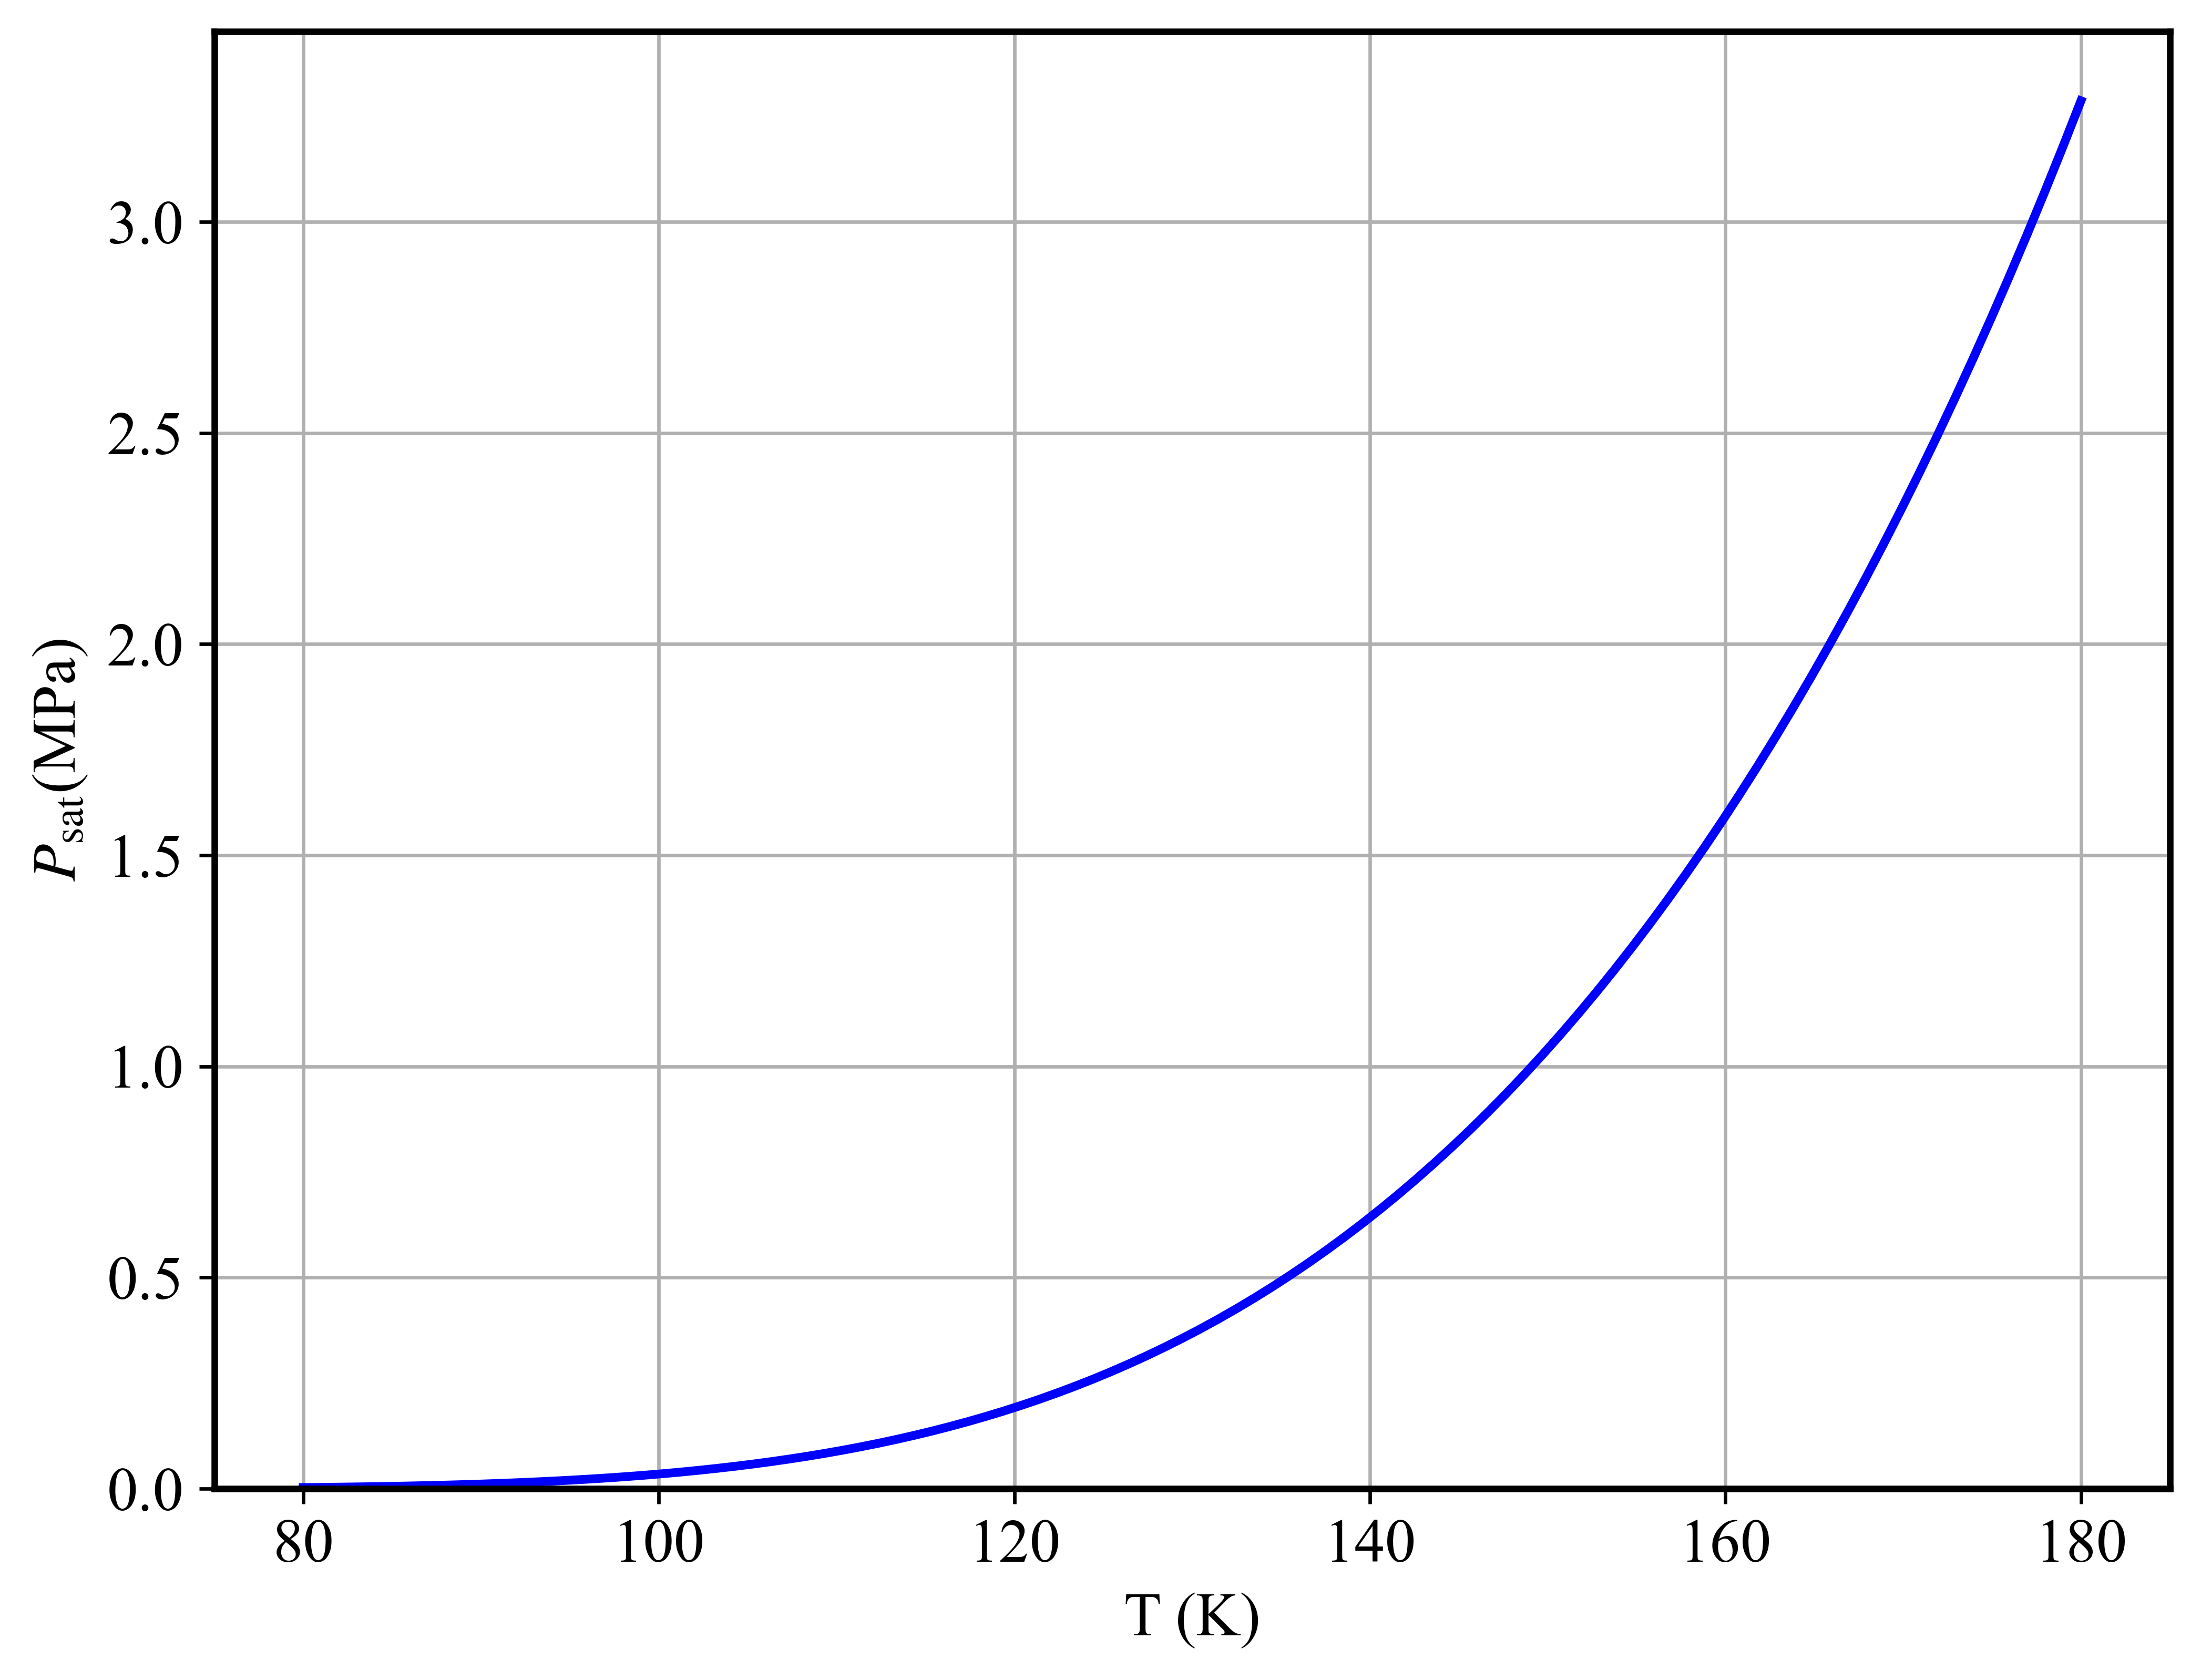
\includegraphics[width=0.7\textwidth]{../chp7/figs/甲烷.png}
    \caption{甲烷的蒸汽压曲线}
\end{figure}
\begin{figure}[H]
    \centering
    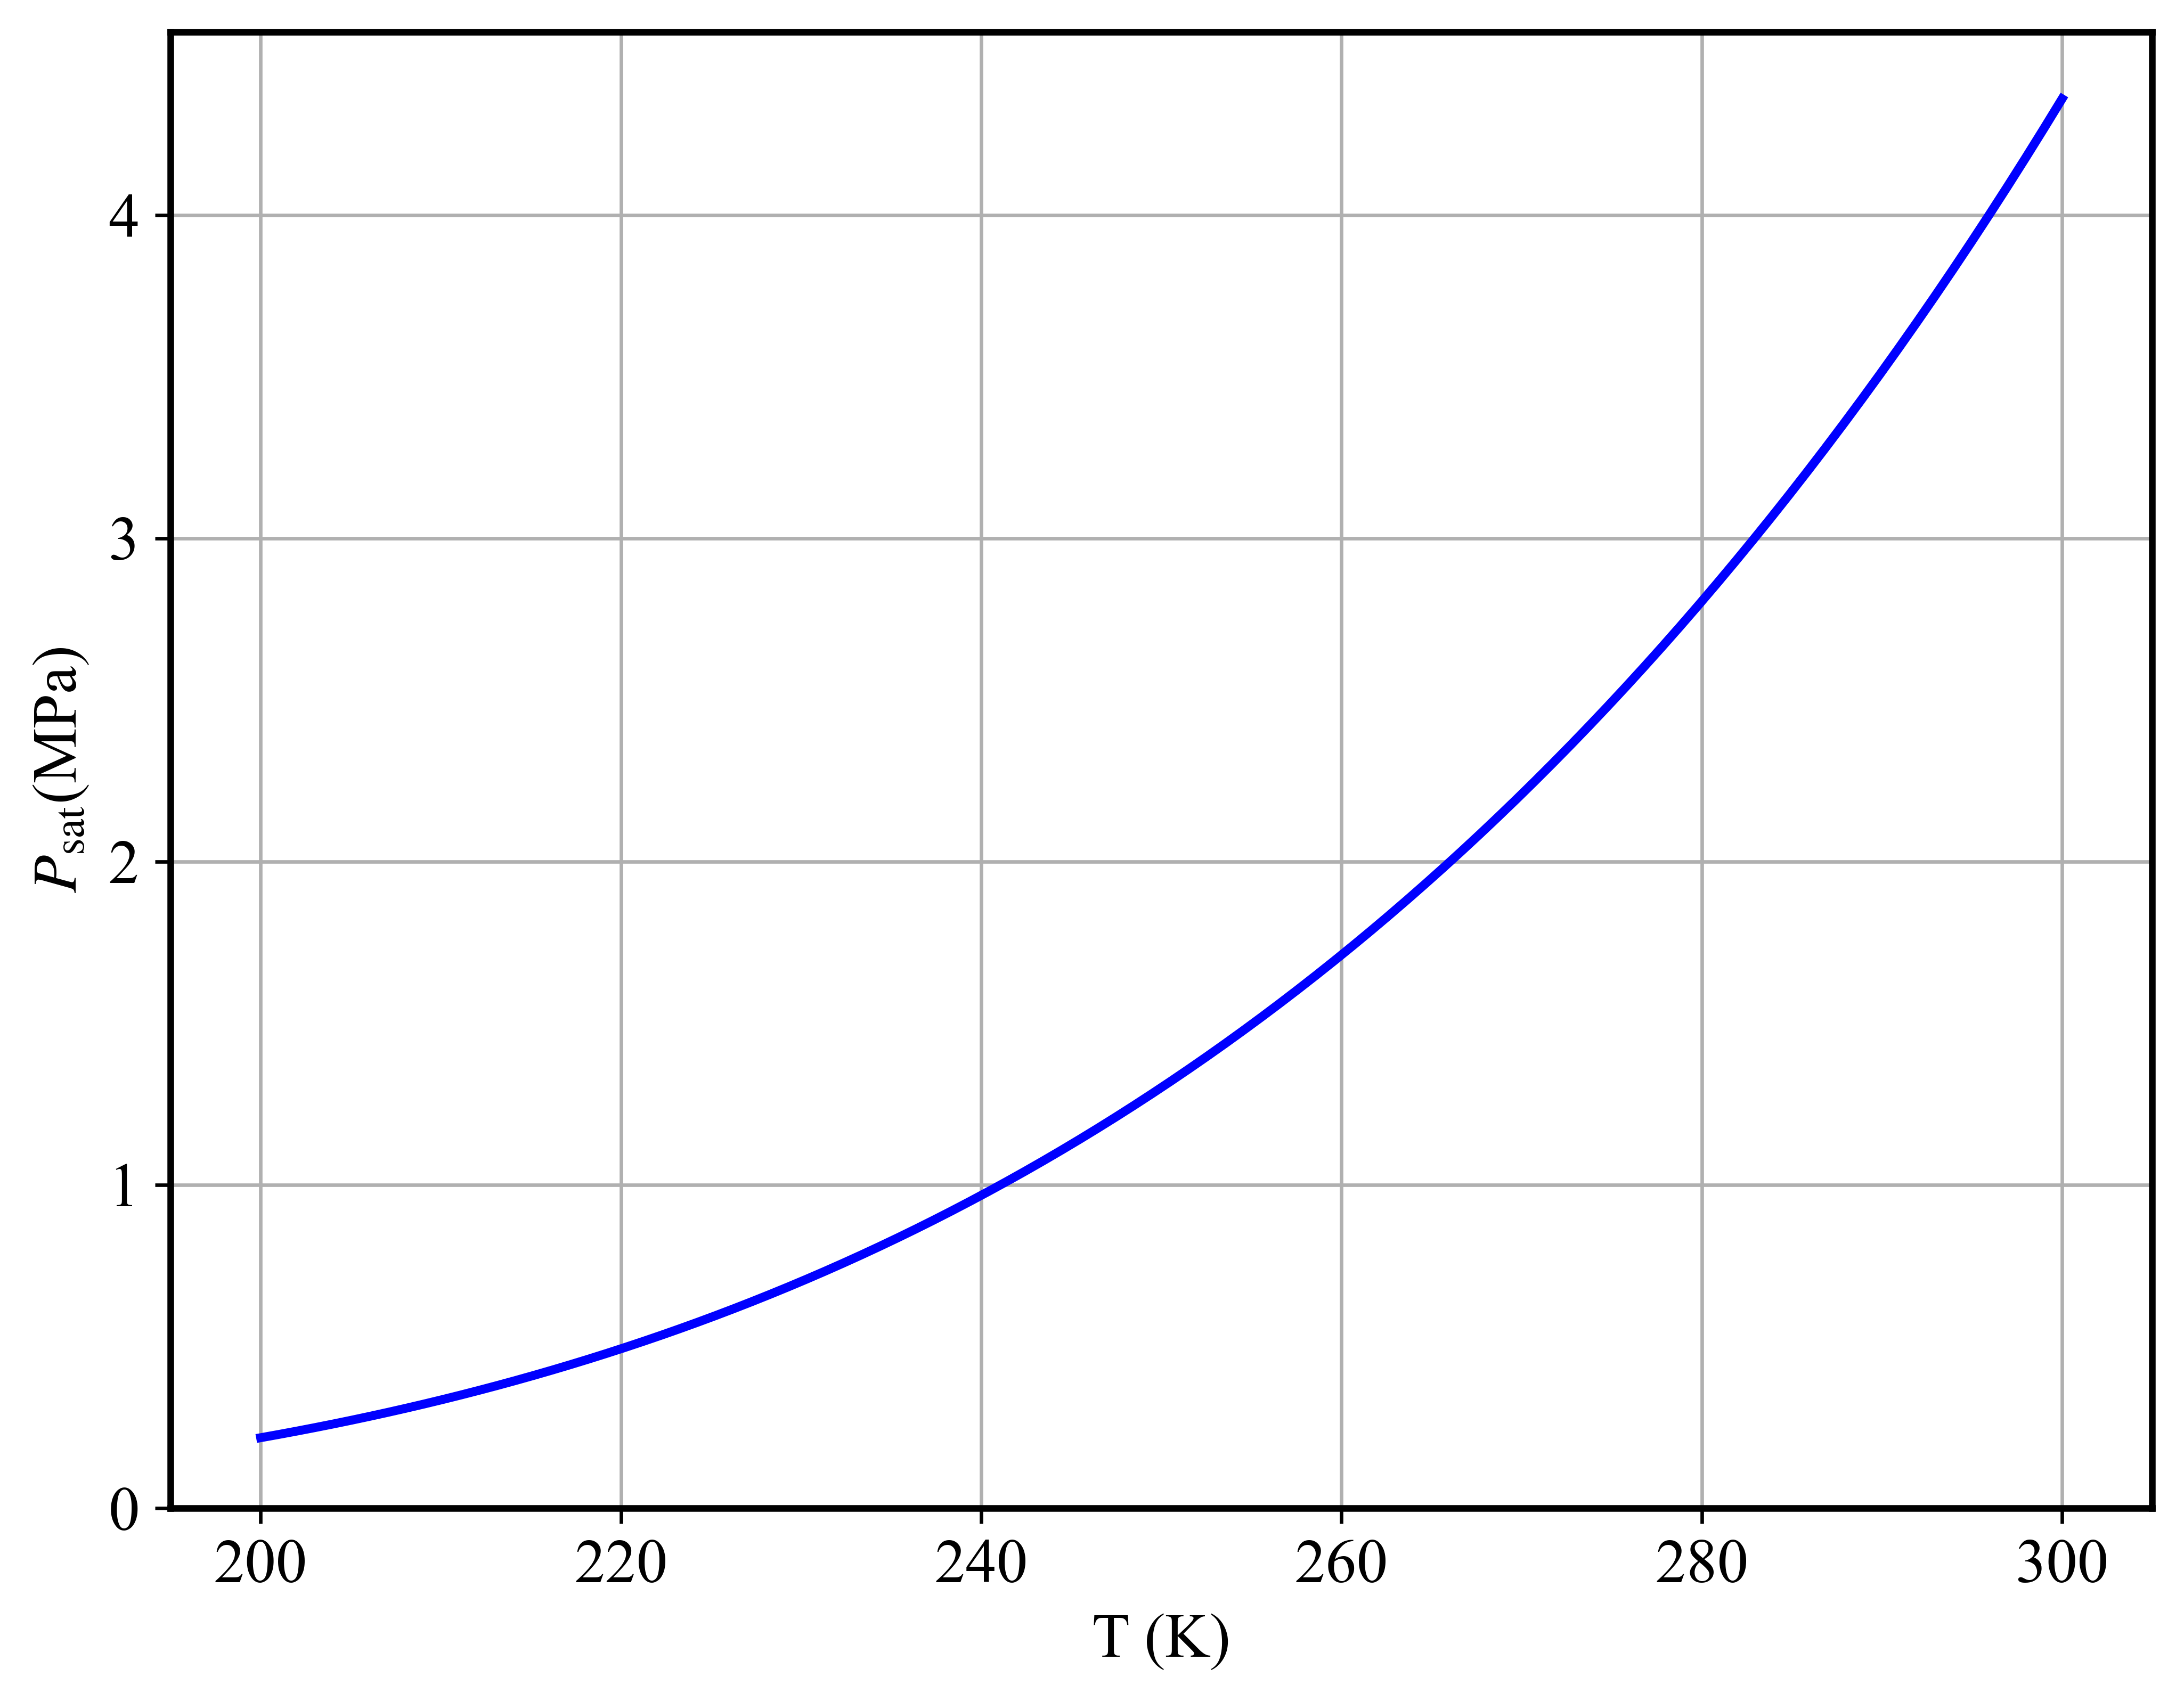
\includegraphics[width=0.7\textwidth]{../chp7/figs/乙烷.png}
    \caption{乙烷的蒸汽压曲线}
\end{figure}
\begin{figure}[H]
    \centering
    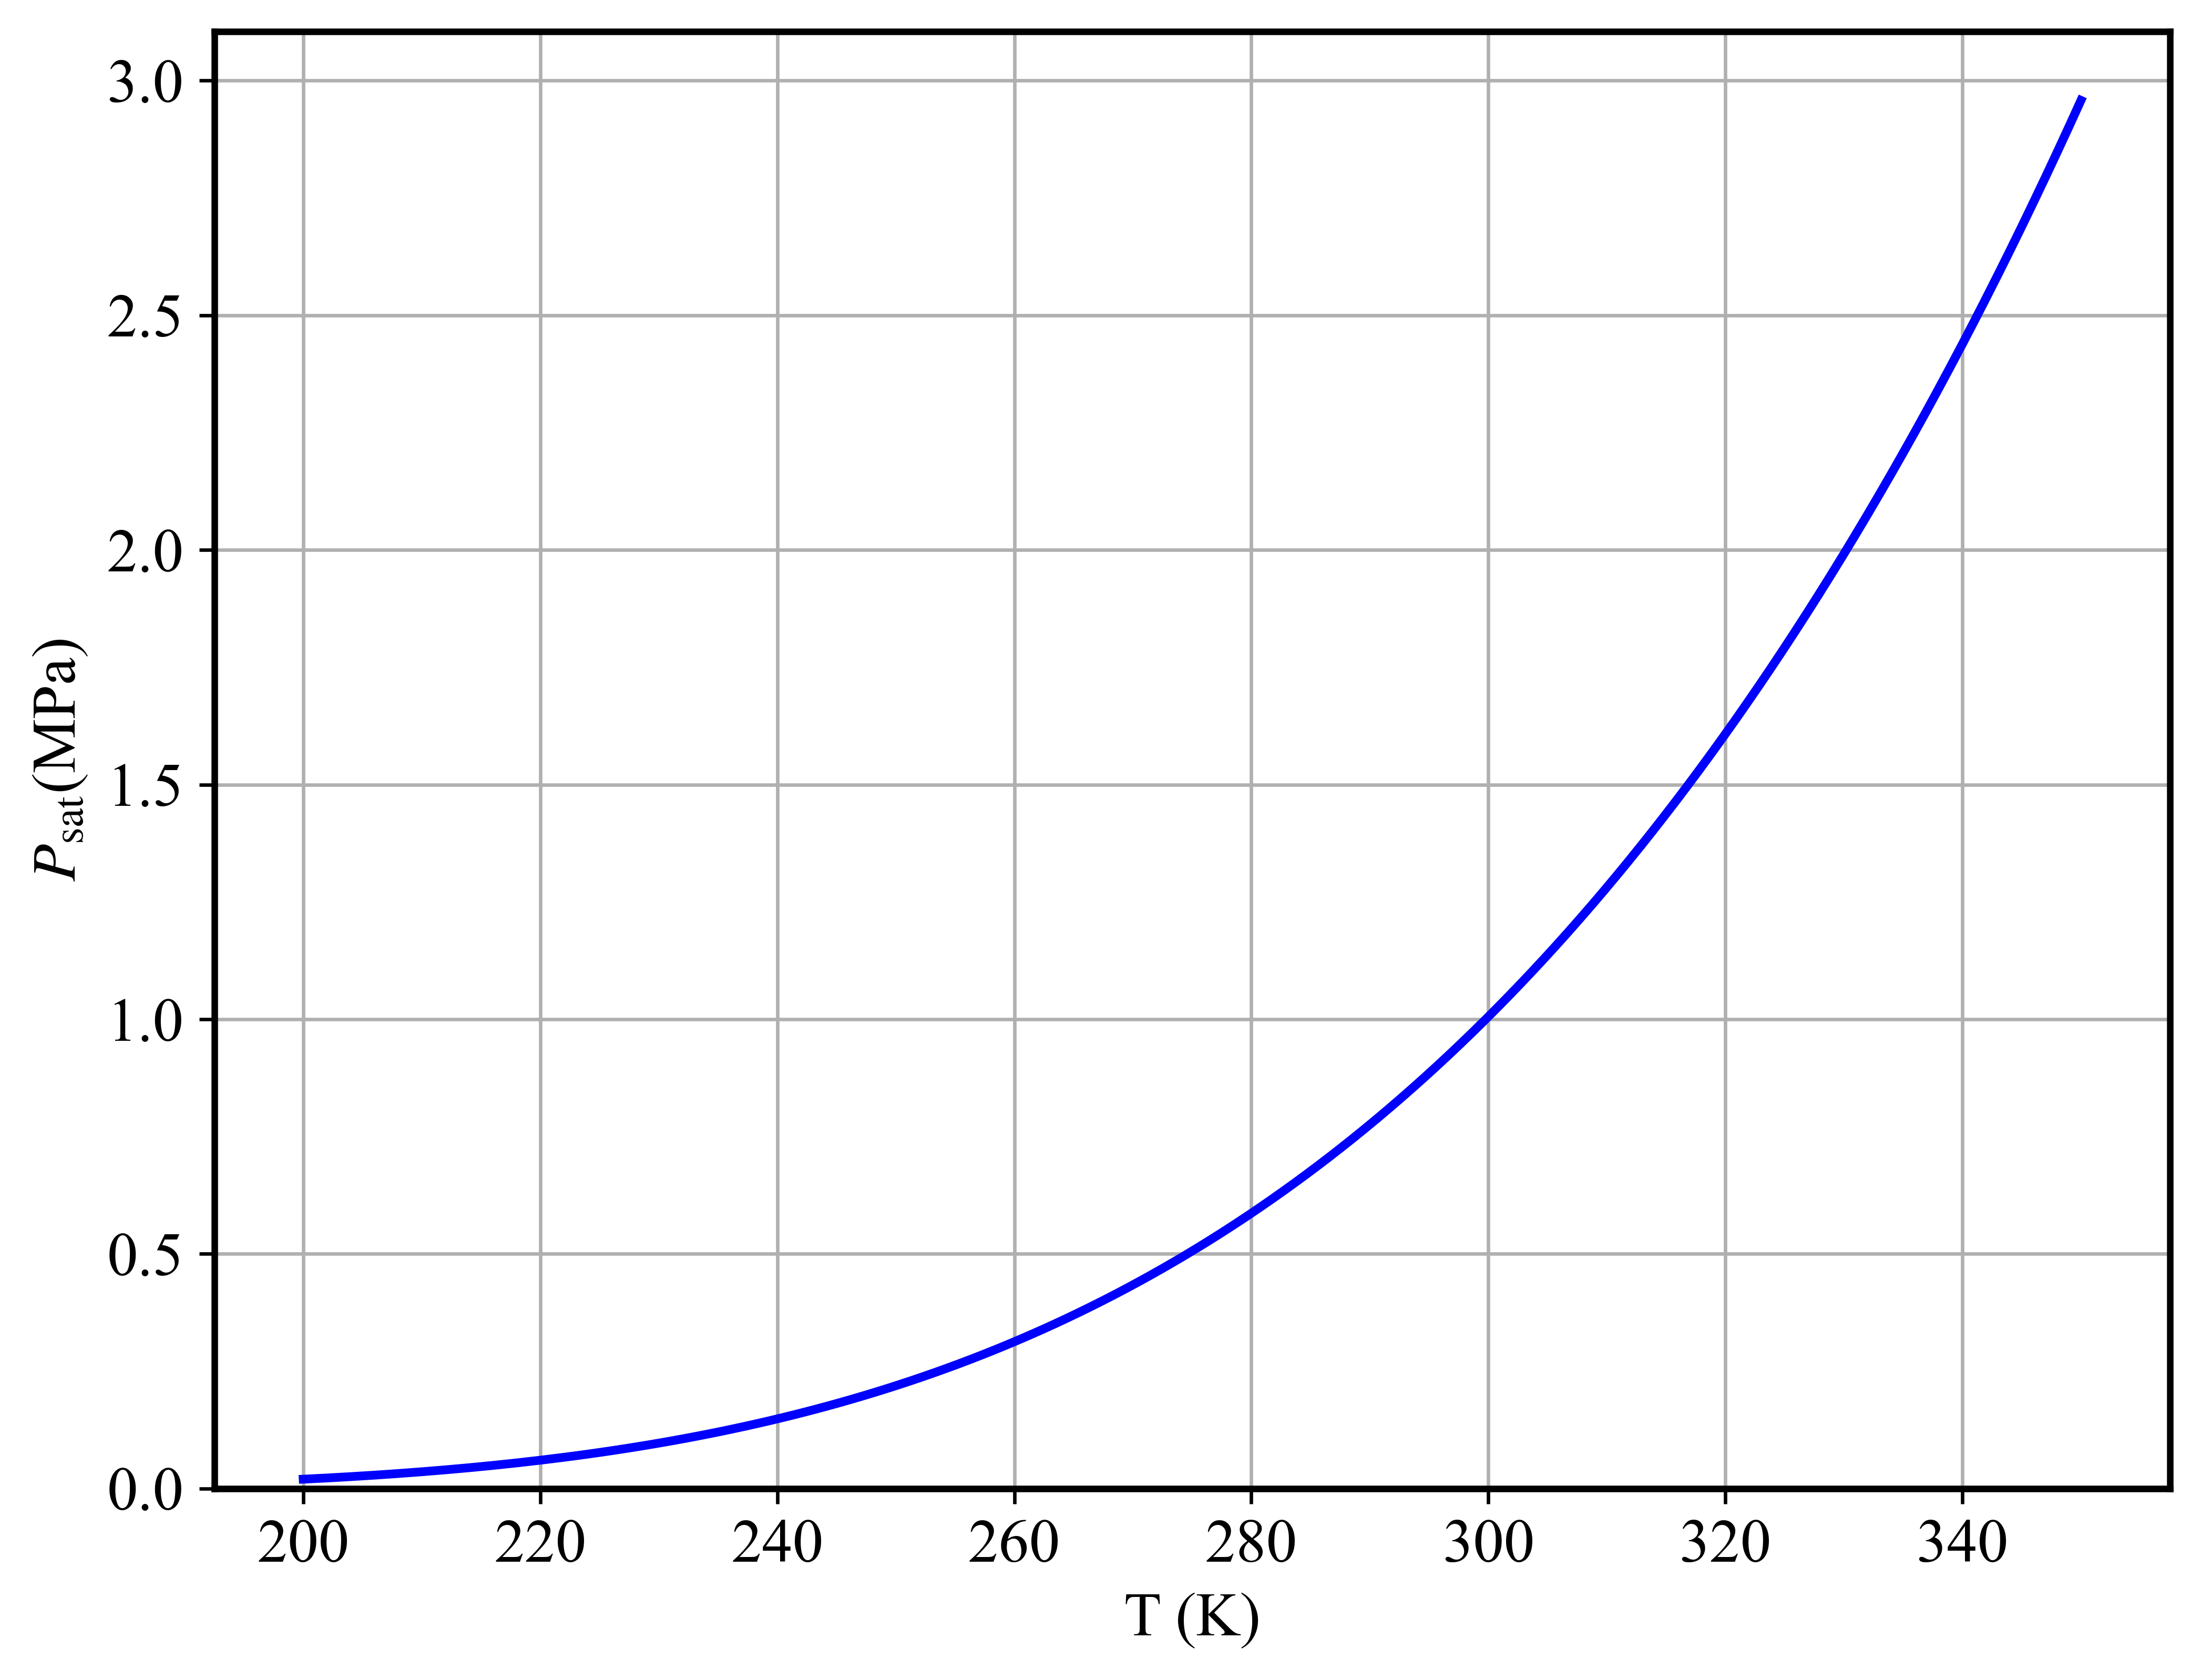
\includegraphics[width=0.7\textwidth]{../chp7/figs/丙烷.png}
    \caption{丙烷的蒸汽压曲线}
\end{figure}
\begin{figure}[H]
    \centering
    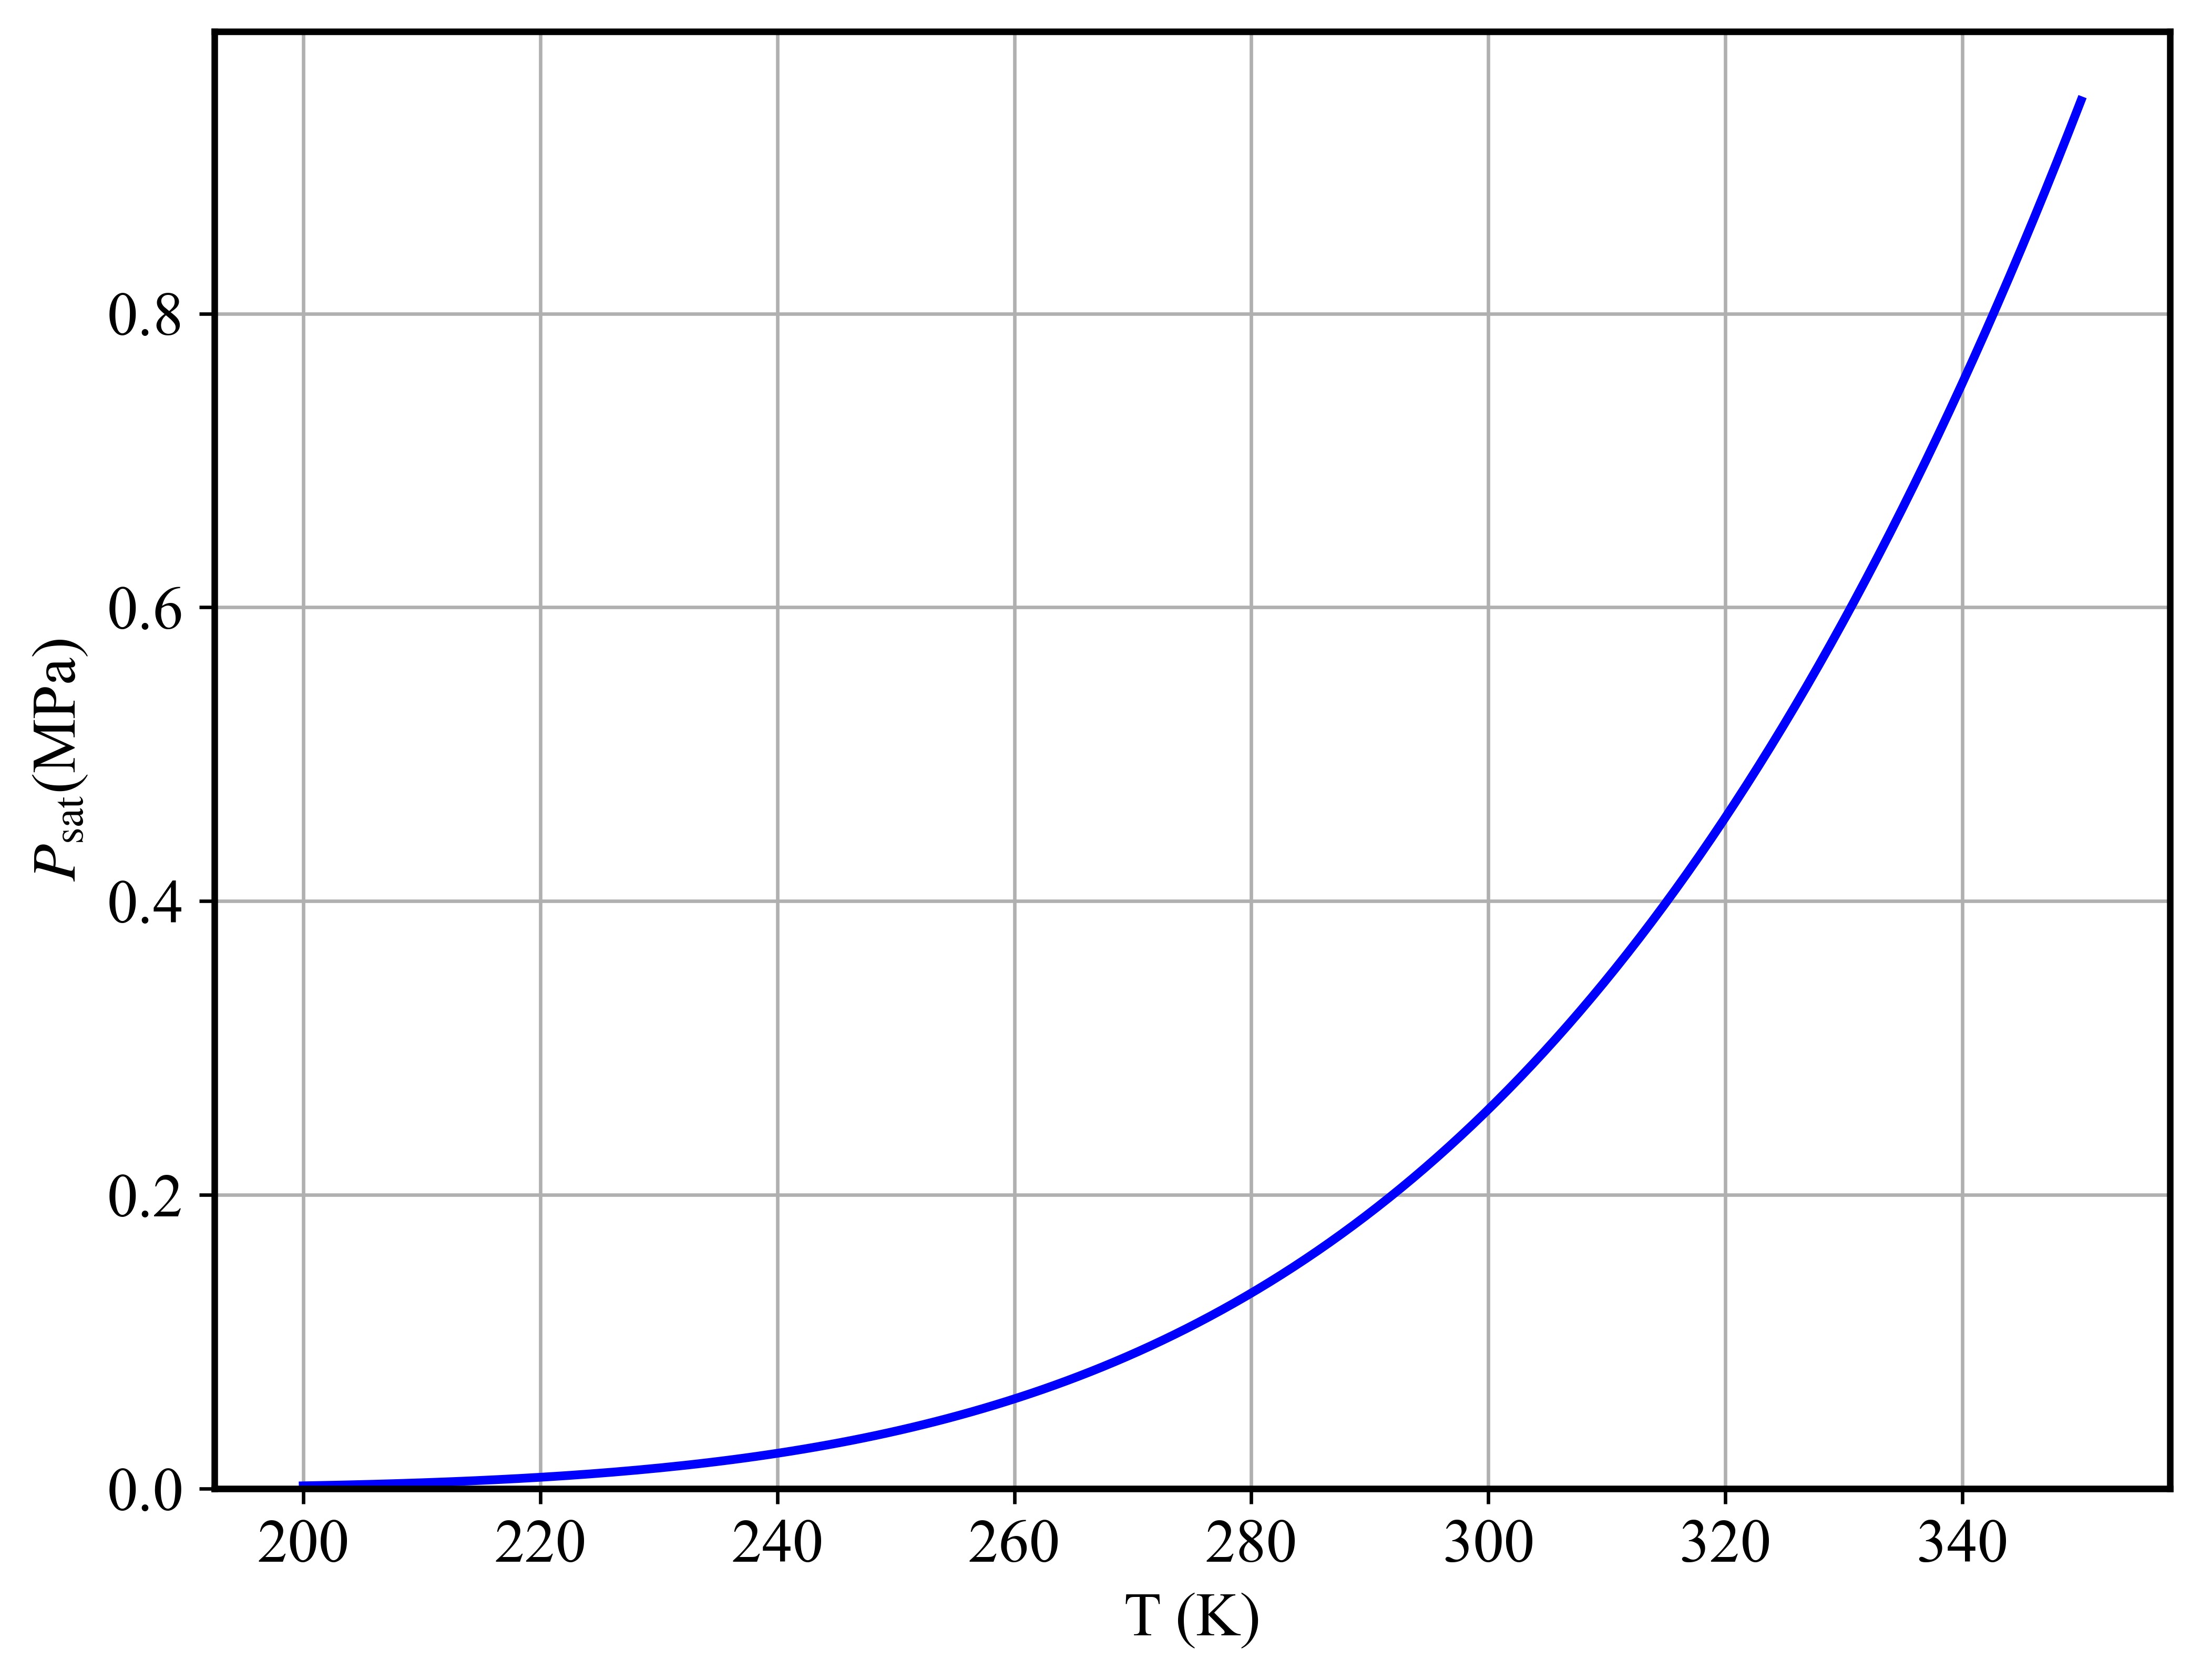
\includegraphics[width=0.7\textwidth]{../chp7/figs/丁烷.png}
    \caption{丁烷的蒸汽压曲线}
\end{figure}

程序如下:
\begin{lstlisting}
import numpy as np
import matplotlib.pyplot as plt
import os

# 使用 Times New Roman 作为 matplotlib 全局字体
plt.rcParams["font.family"] = "serif"
plt.rcParams["font.serif"] = ["Times New Roman"]
plt.rcParams["mathtext.fontset"] = "stix"
plt.rcParams["font.size"] = 14  # 增大全局字体
plt.rcParams["axes.linewidth"] = 1.5  # 增粗坐标轴


class PR73:
    def __init__(self, Tc, pc, A1, A2, A3):
        self.Tc = Tc  # K
        self.pc = pc * 1e6  # Pa,输入MPa
        self.A1 = A1
        self.A2 = A2
        self.A3 = A3

    def psat(self, T):
        Tr = T / self.Tc
        p = self.pc * (Tr) ** (
            self.A1 + self.A2 * (1 - Tr) ** 1.89 + self.A3 * (1 - Tr) ** 5.67
        )
        return p / 1e6  # 输出MPa

    def plot_psat(self, fluid_name, Tmin, Tmax, nt):
        T_grid = np.linspace(Tmin, Tmax, nt)
        psat_grid = np.zeros(nt)
        for i, T in enumerate(T_grid):
            psat_grid[i] = self.psat(T)

        base_dir = os.path.dirname(os.path.abspath(__file__))
        fig_dir = os.path.join(base_dir, "figs")
        os.makedirs(fig_dir, exist_ok=True)

        fig = plt.figure(figsize=(8, 6))
        ax = fig.add_subplot(1, 1, 1)
        ax.plot(T_grid, psat_grid, "b-", linewidth=2)
        ax.set_ylim(bottom=0)
        ax.set_xlabel("T (K)", fontsize=14)
        ax.set_ylabel(r"$P_\mathrm{sat}$(MPa)", fontsize=14)
        ax.grid(True)

        # 保存图像
        savepath = os.path.join(fig_dir, f"{fluid_name}.png")
        fig.savefig(savepath, dpi=600, bbox_inches="tight", transparent=False)
        plt.close(fig)


CH4 = PR73(190.551, 4.5992, 5.87304544, 6.23280143, 13.0721578)
CH4.plot_psat("甲烷", 80, 180, 100)
C2H6 = PR73(305.33, 4.8717, 6.30717658, 7.47042131, 17.0958137)
C2H6.plot_psat("乙烷", 200, 300, 100)
C3H8 = PR73(369.80, 4.239, 6.50580501, 8.6776247, 18.0116214)
C3H8.plot_psat("丙烷", 200, 350, 150)
C4H10 = PR73(425.2, 3.8, 6.81692028, 8.77671813, 23.7680492)
C4H10.plot_psat("丁烷", 200, 350, 150)
\end{lstlisting}

\subsection*{7-4}
制冷剂R290、R600a、R1234yf和R1234ze(E)的p-T相图如下所示:
\begin{figure}[H]
    \centering
    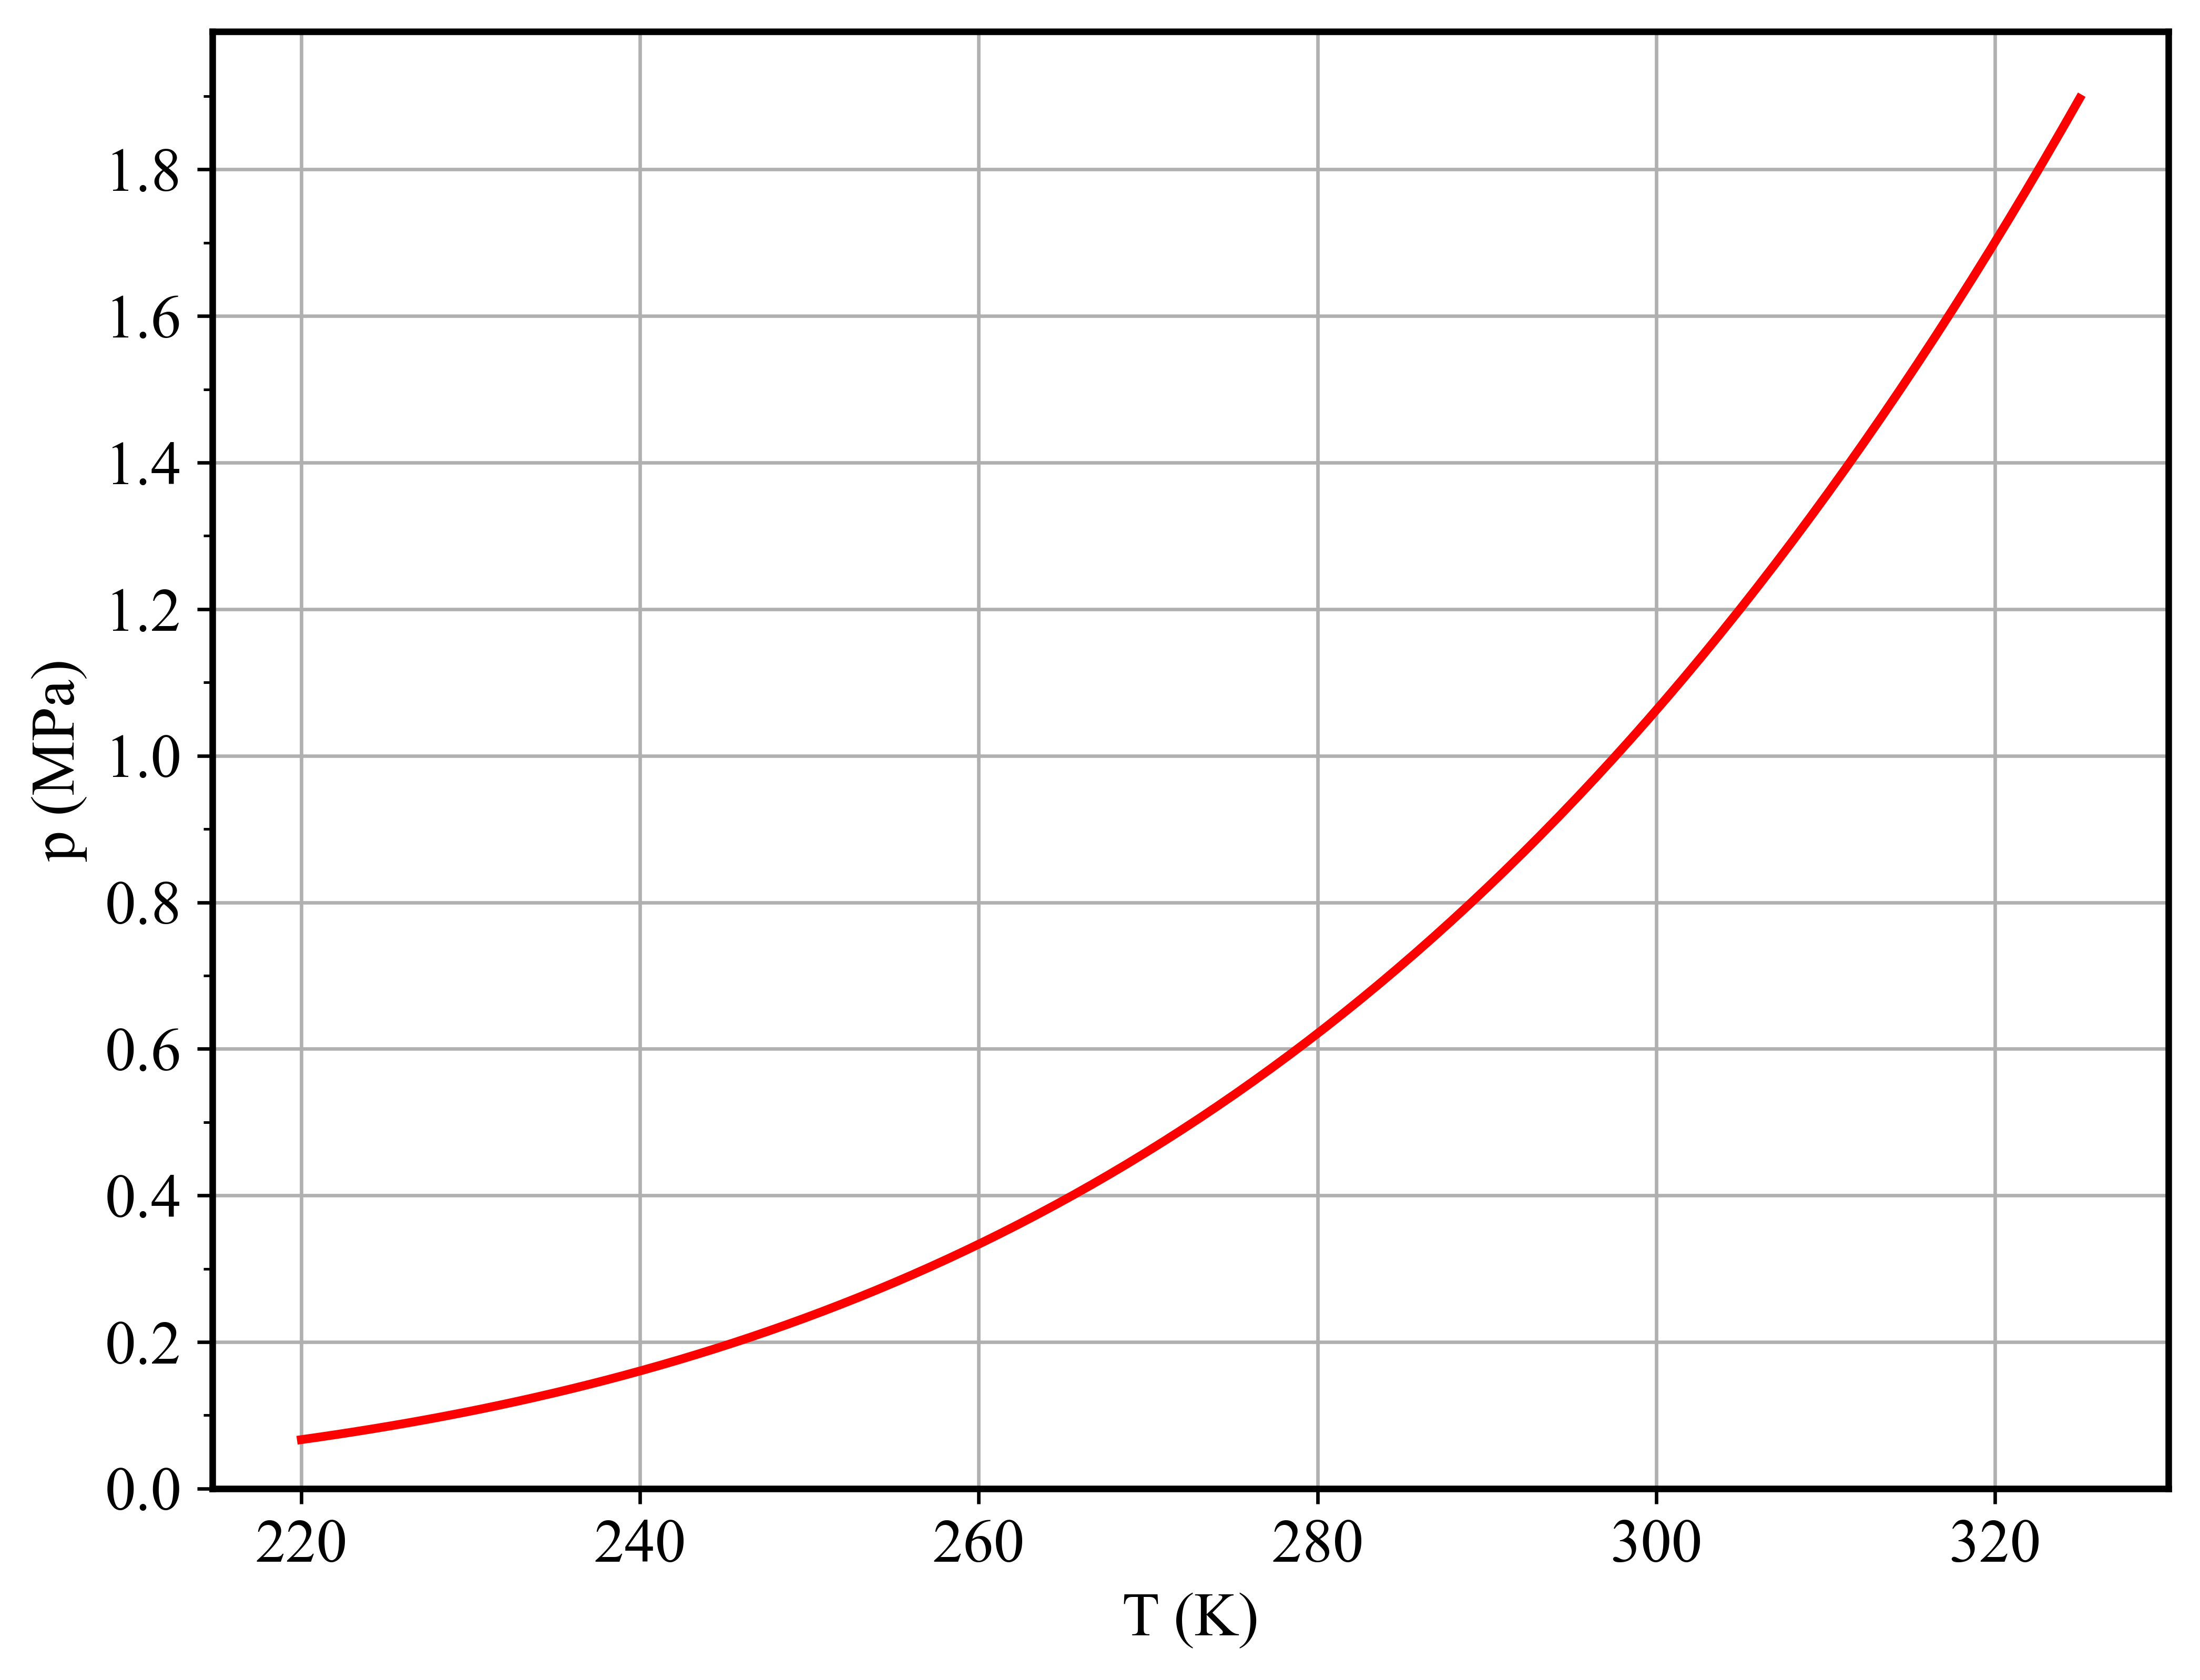
\includegraphics[width=0.7\textwidth]{../chp7/figs/R290_pT.png}
    \caption{R290的p-T相图}
\end{figure}
\begin{figure}[H]
    \centering
    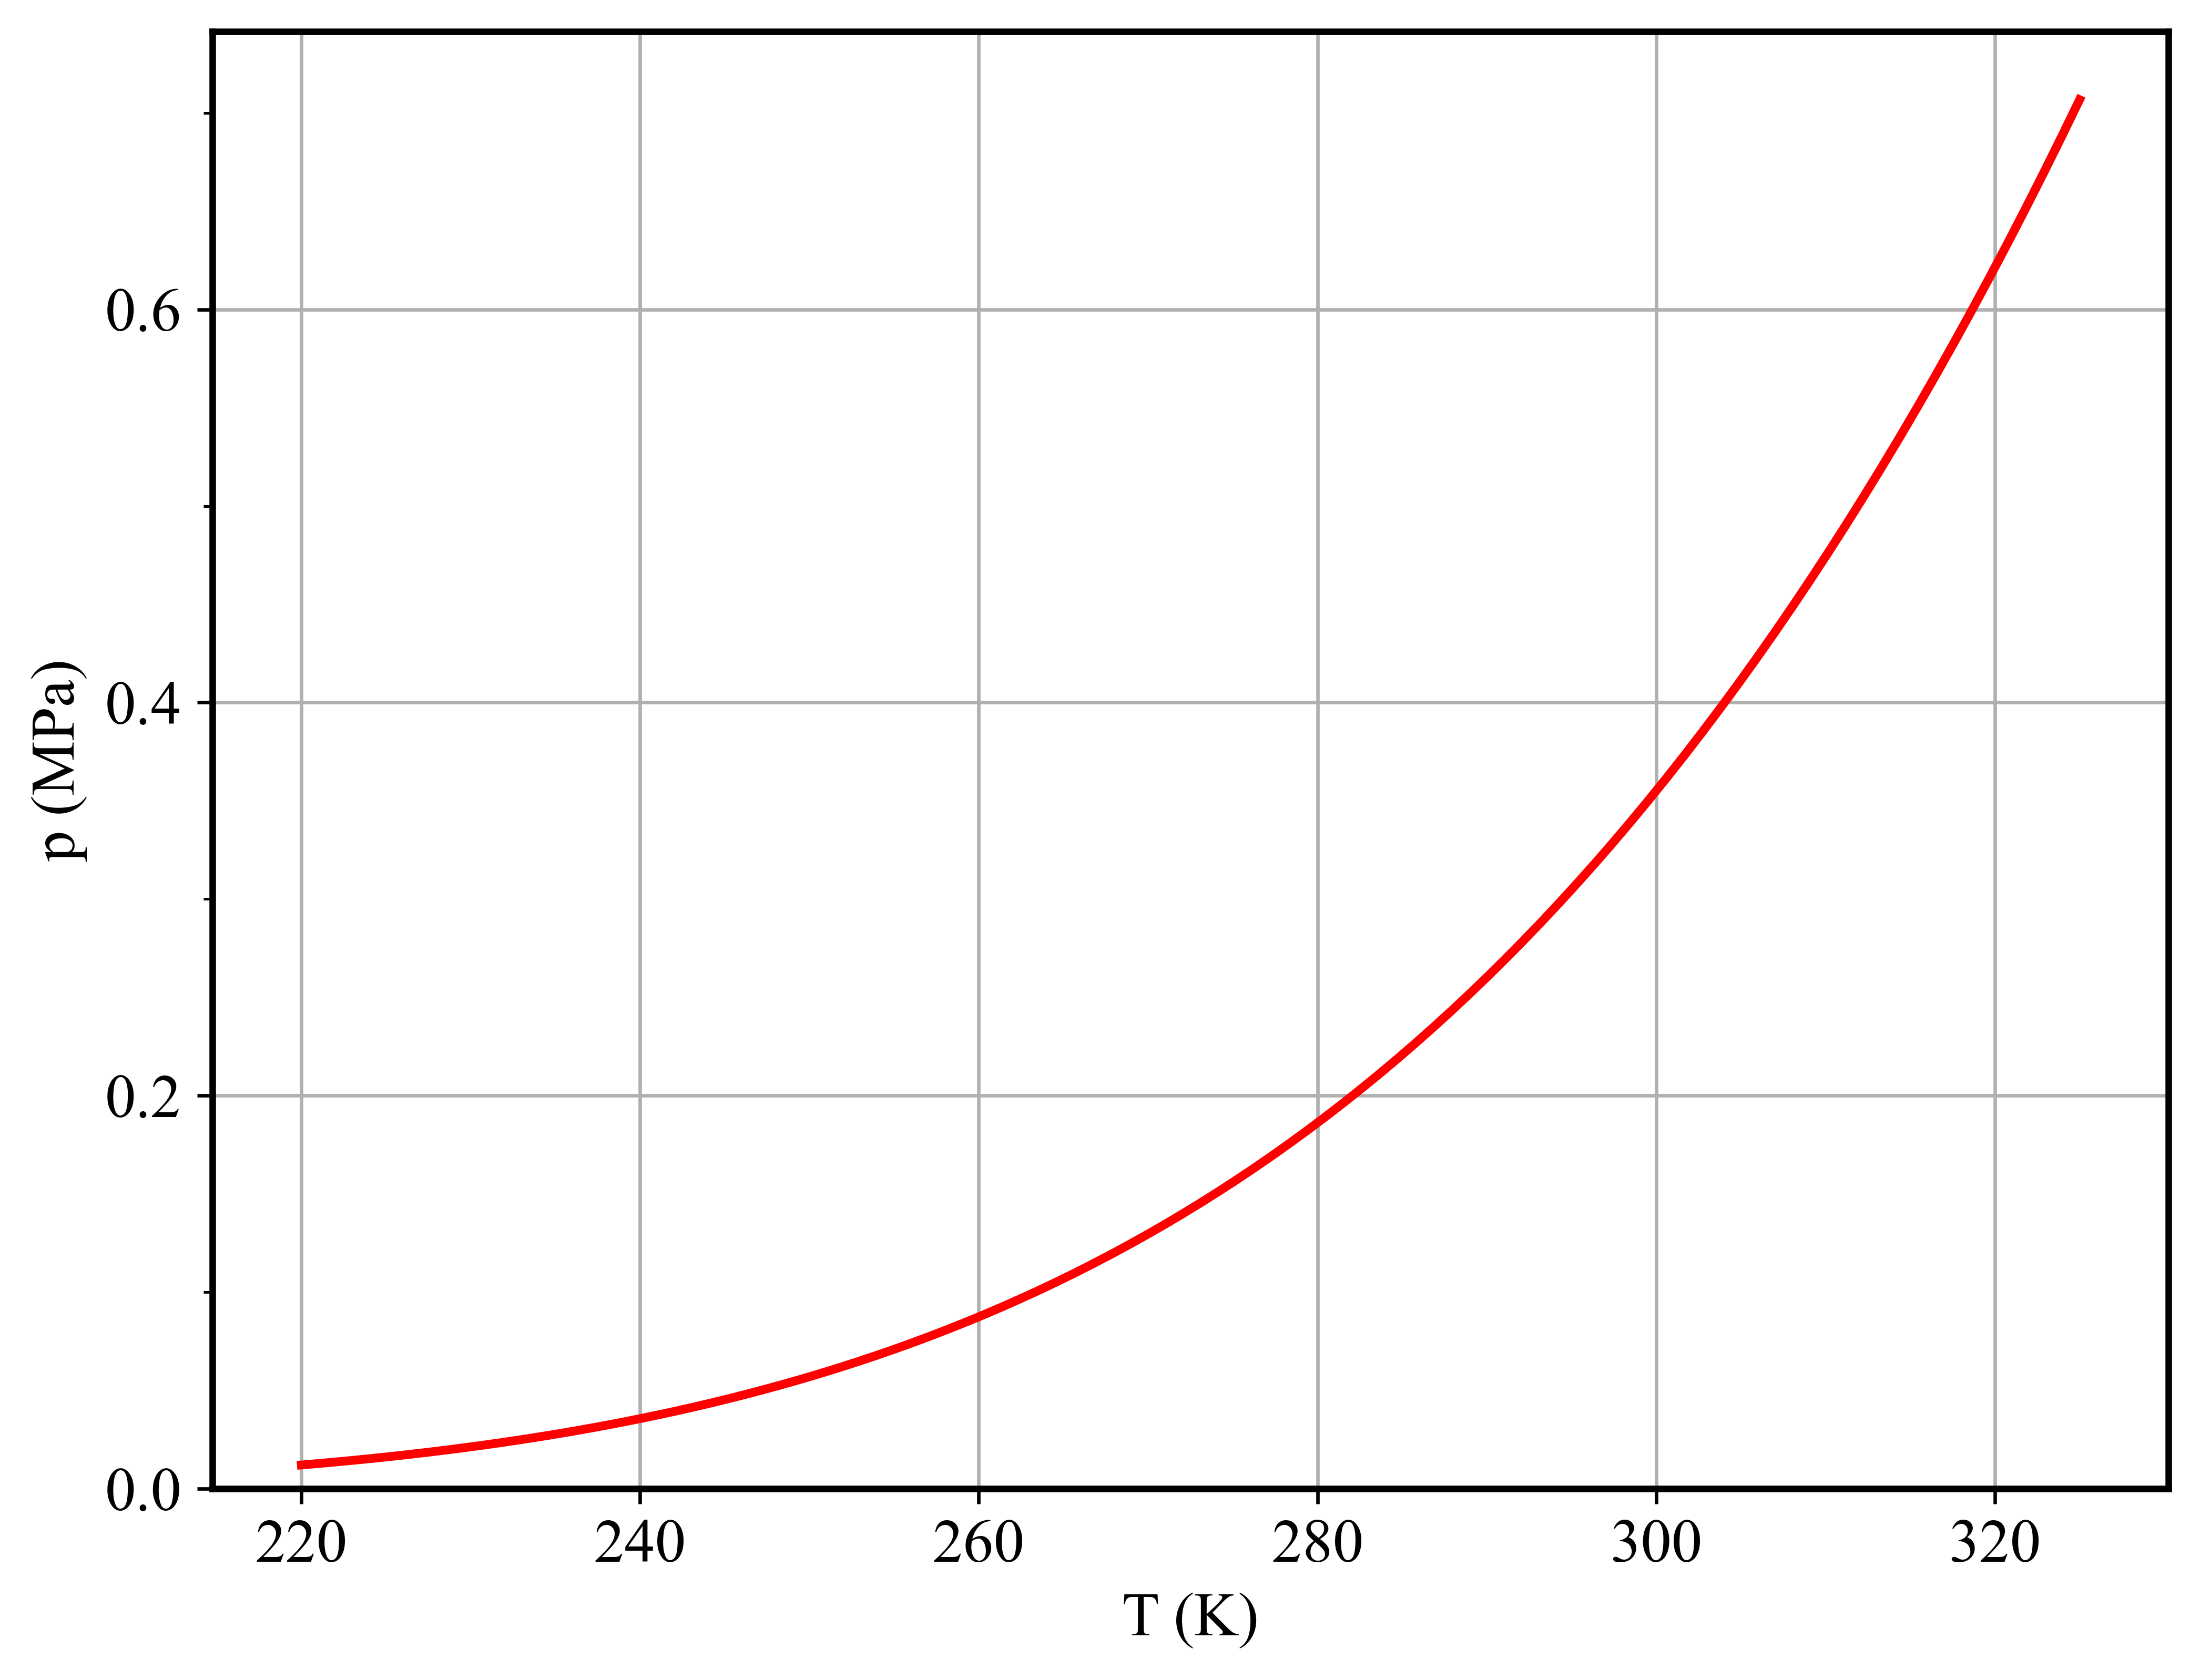
\includegraphics[width=0.7\textwidth]{../chp7/figs/R600a_pT.png}
    \caption{R600a的p-T相图}
\end{figure}
\begin{figure}[H]
    \centering
    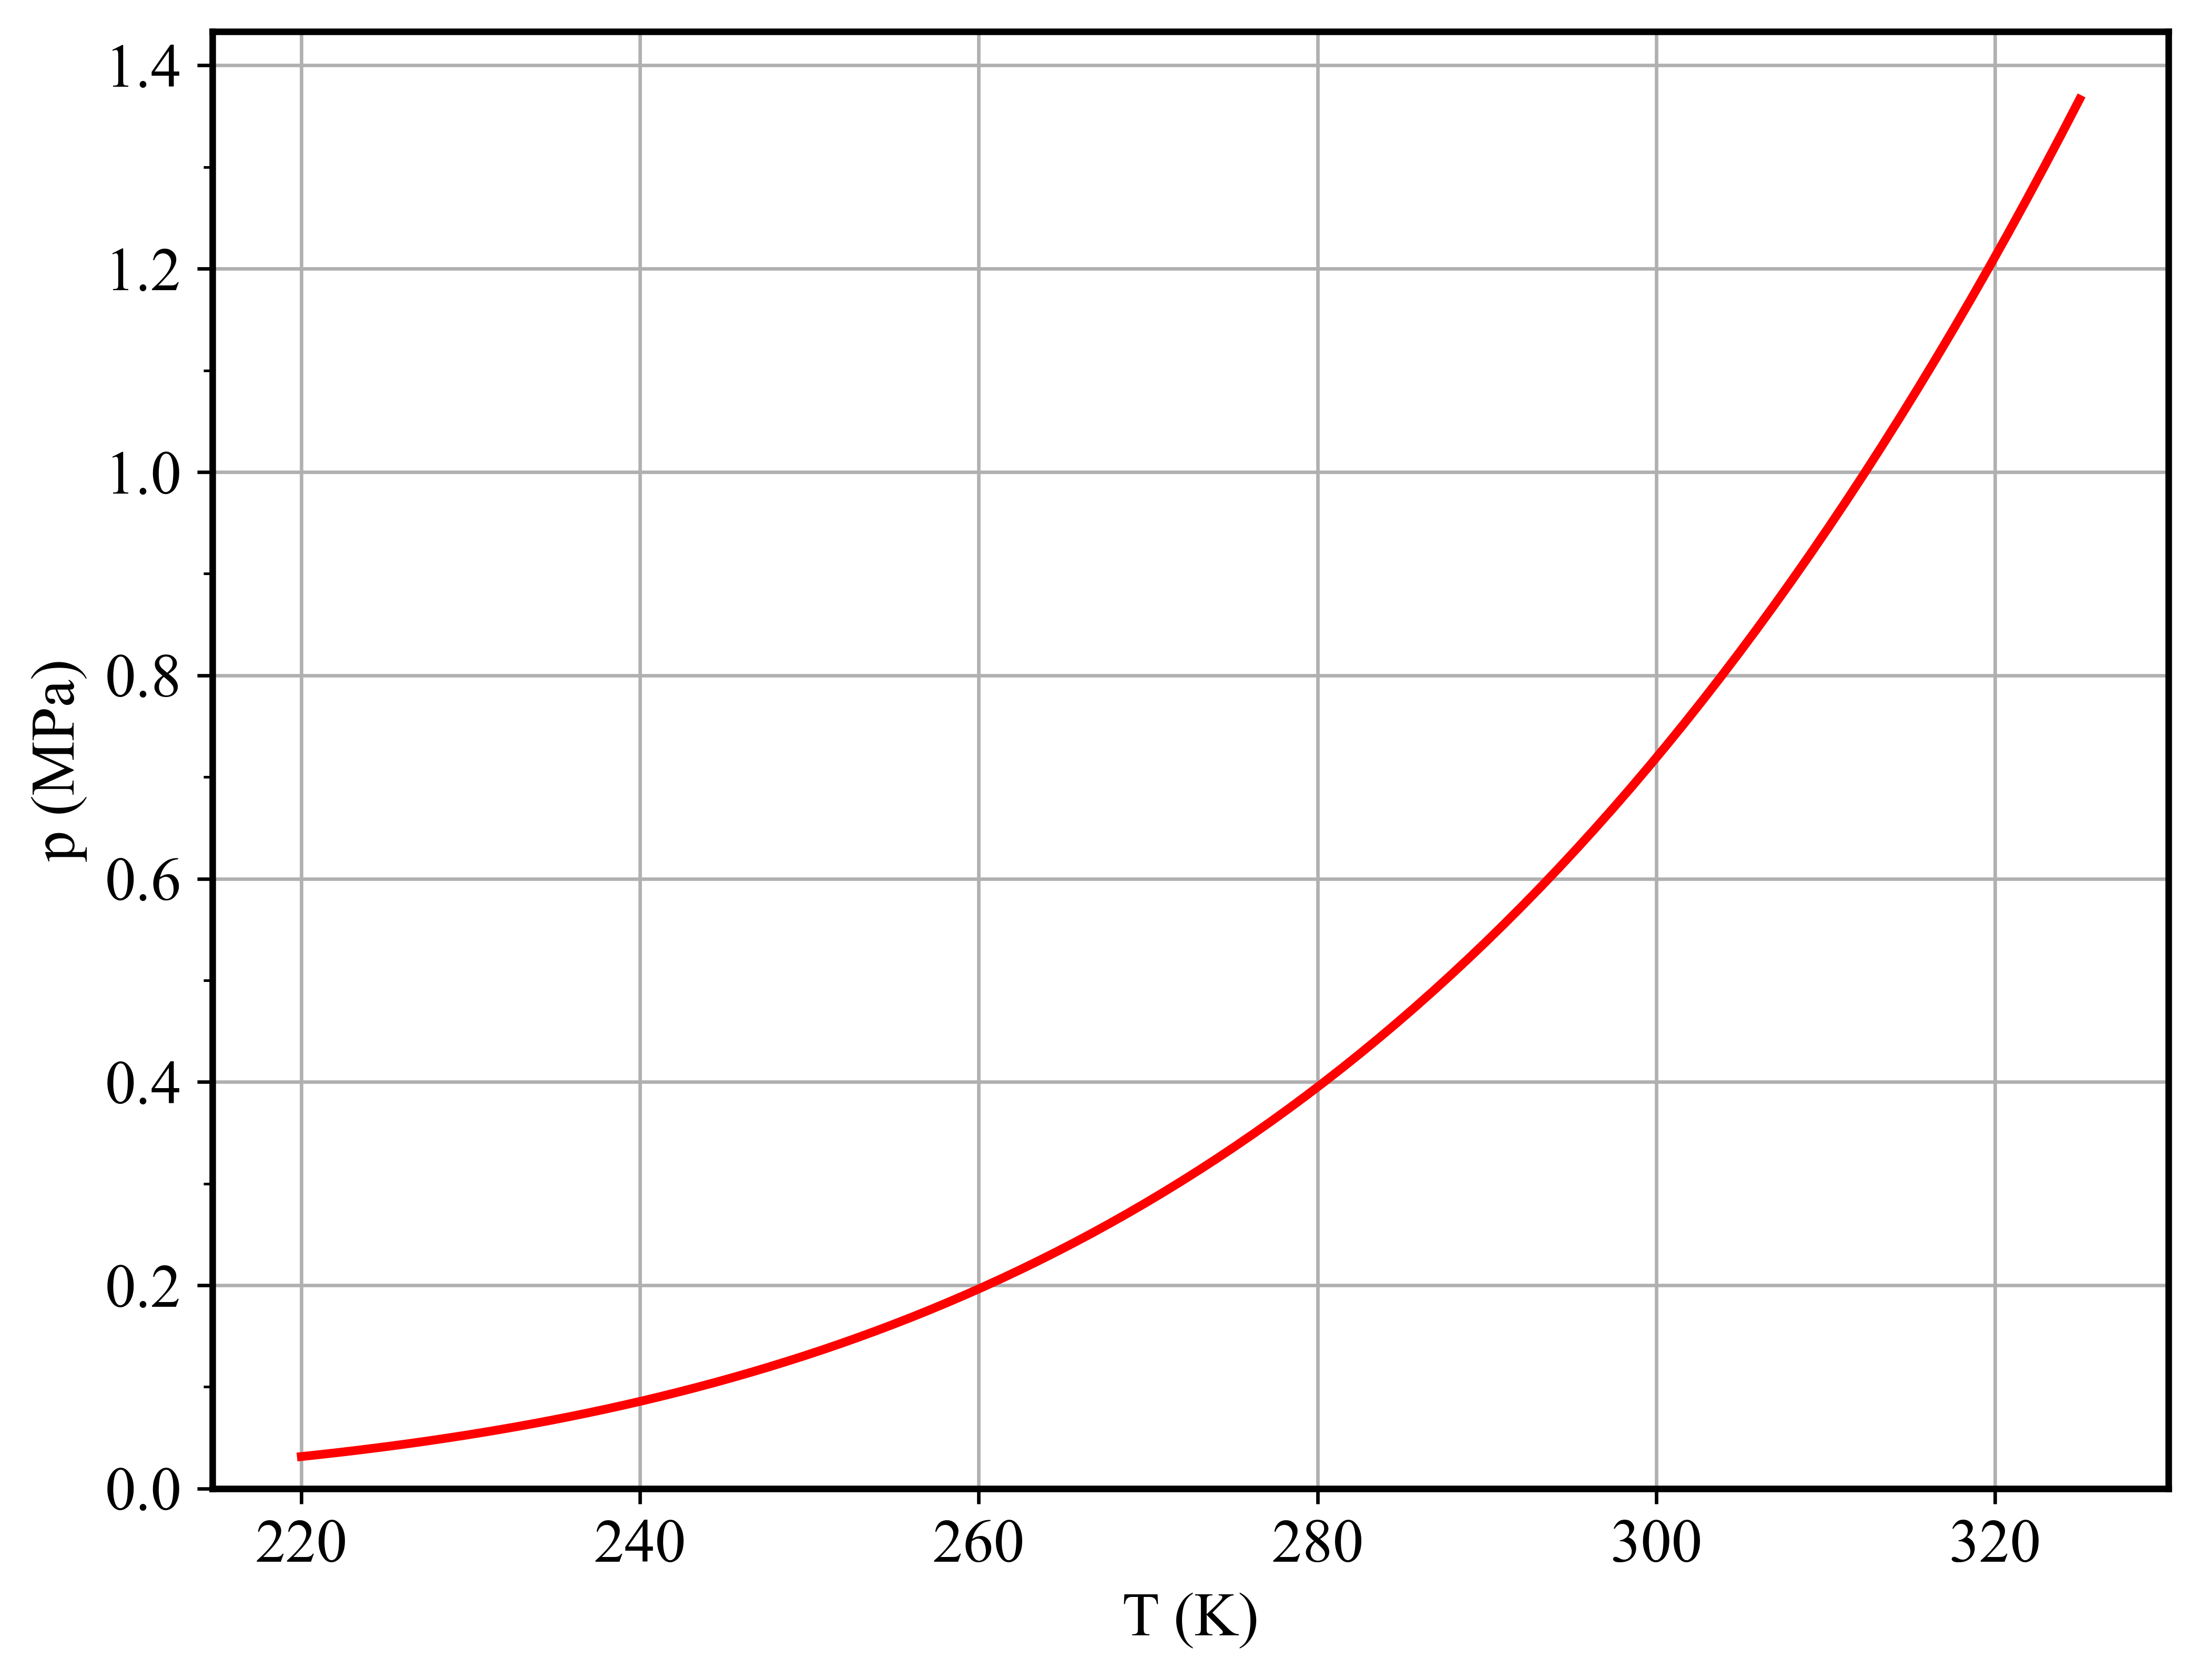
\includegraphics[width=0.7\textwidth]{../chp7/figs/R1234yf_pT.png}
    \caption{R1234yf的p-T相图}
\end{figure}
\begin{figure}[H]
    \centering
    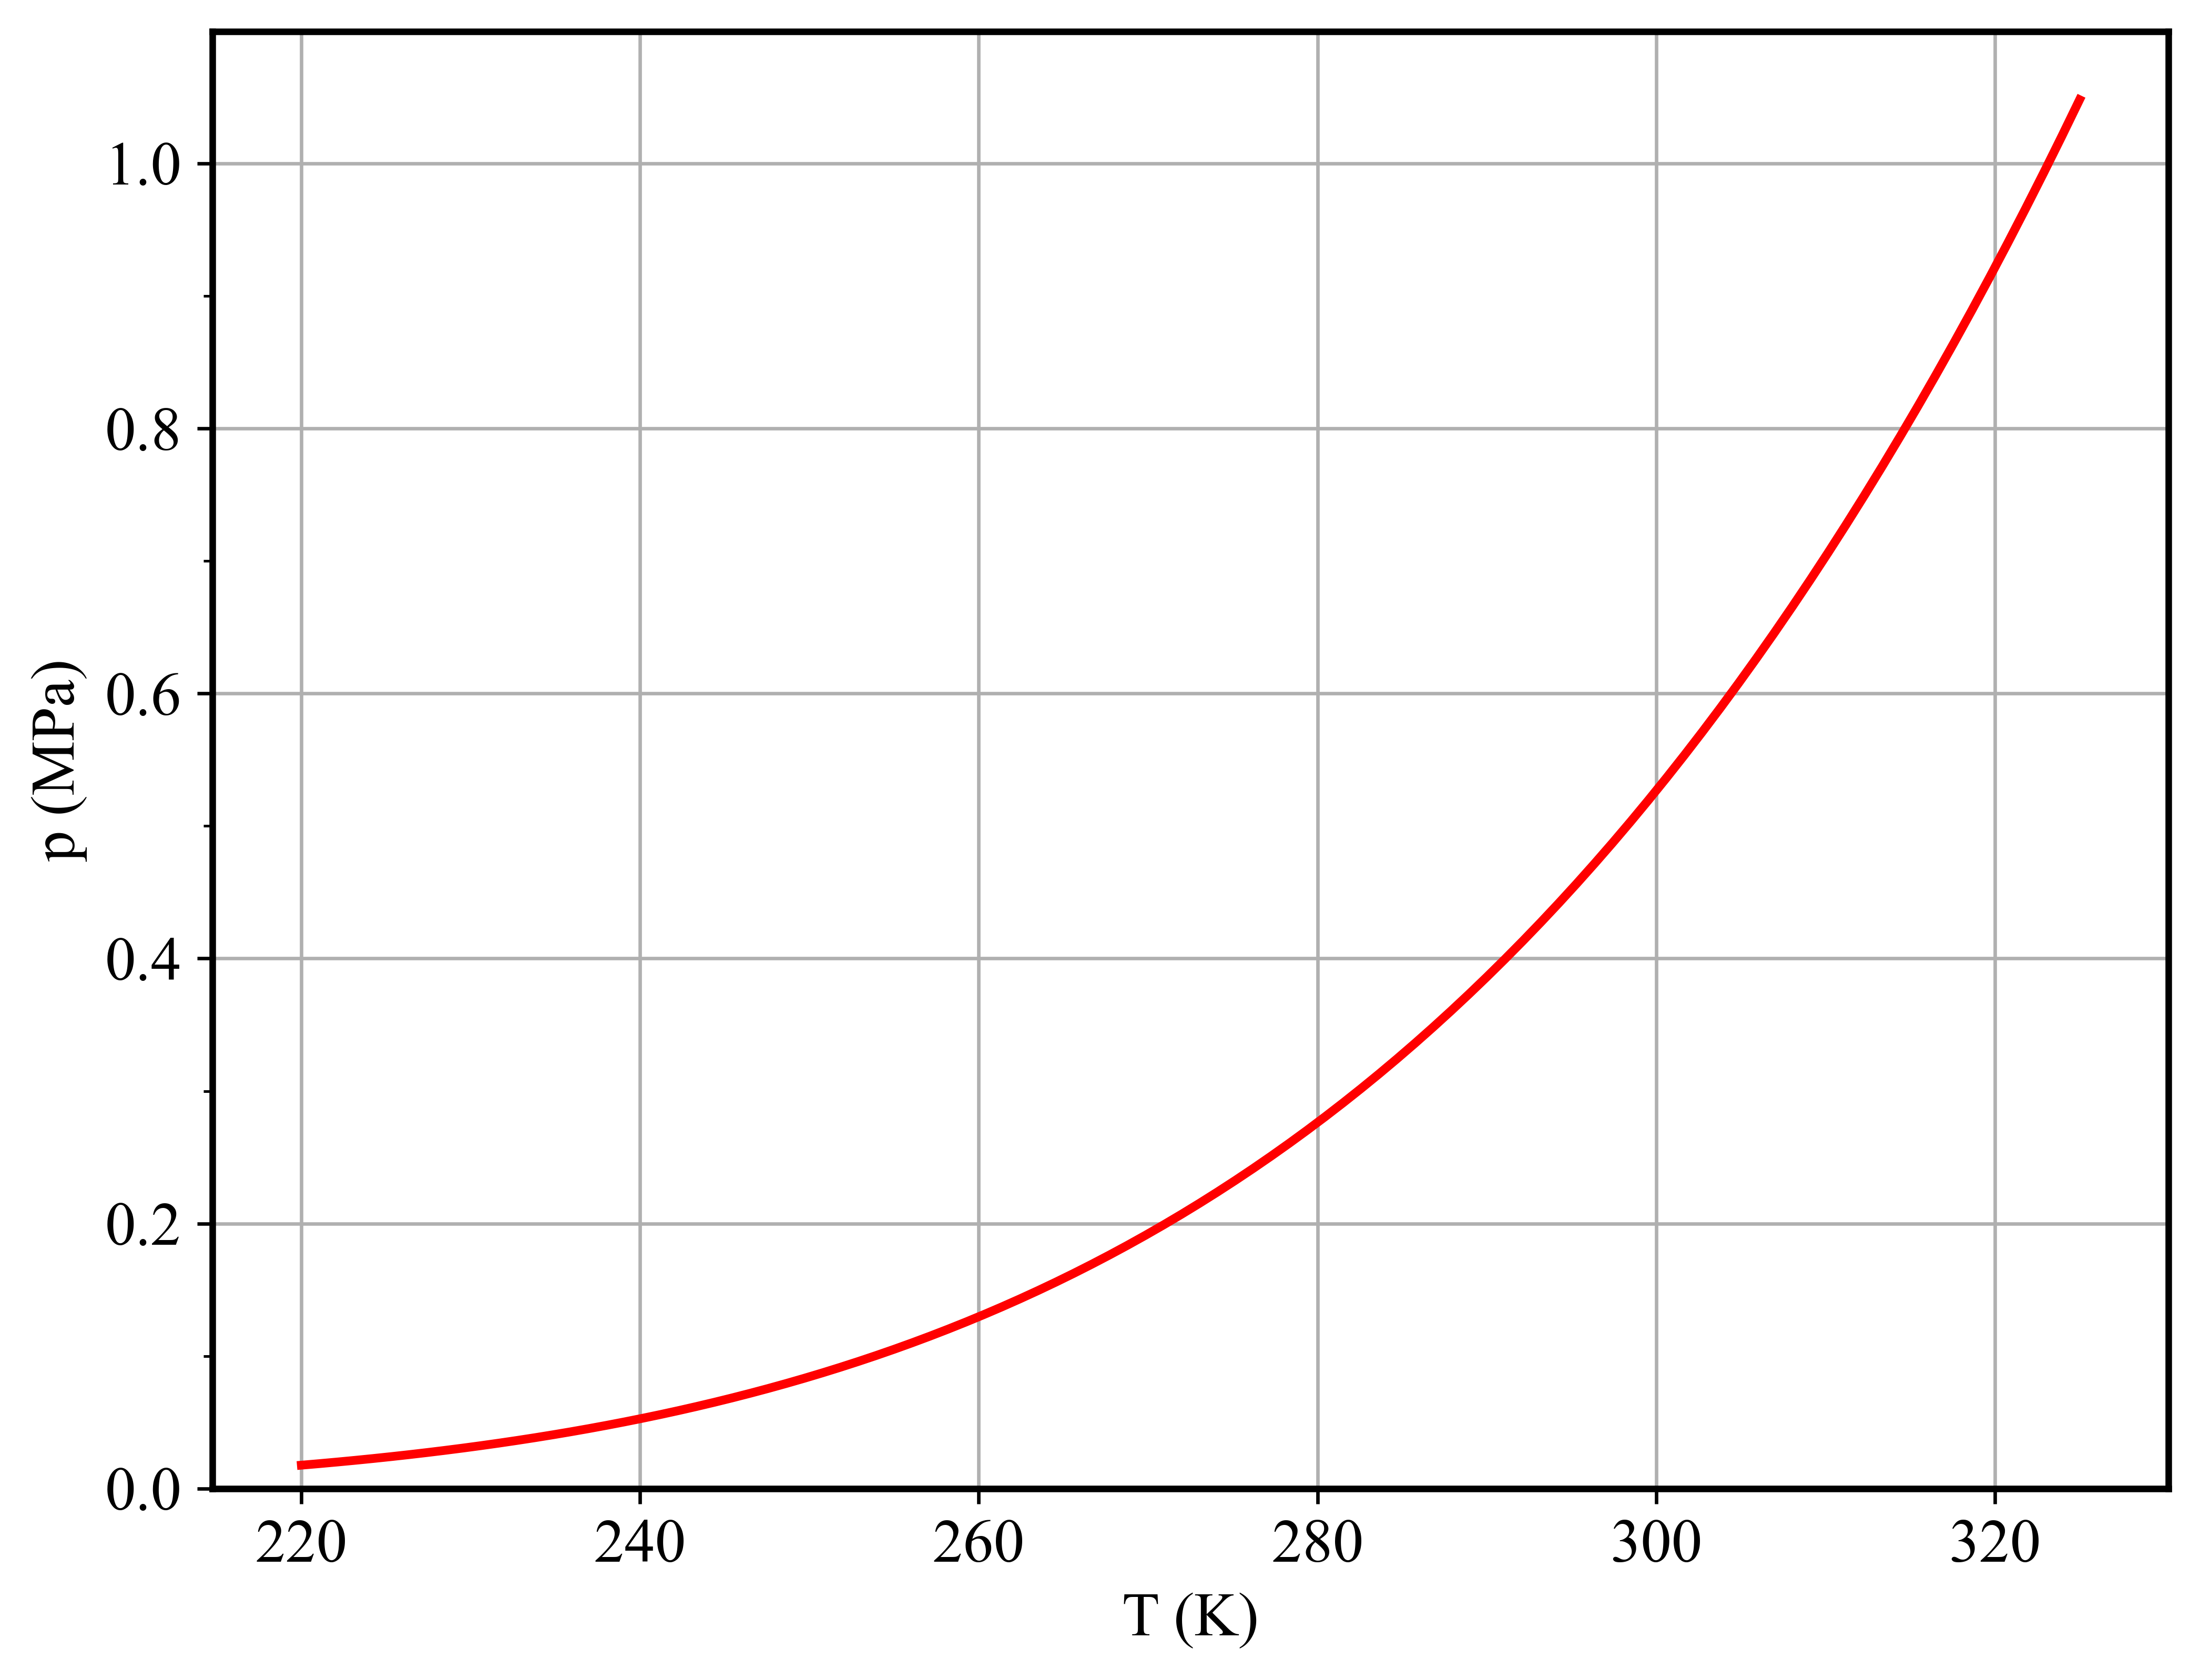
\includegraphics[width=0.7\textwidth]{../chp7/figs/R1234ze(E)_pT.png}
    \caption{R1234ze(E)的p-T相图}
\end{figure}



\subsection*{7-5}



\end{document}